\section{Results}

\subsection{Performance of arm movement controllers}
Different controllers that was made for the motion control of the robot arm was compared when acting on a \(40^{\circ}\) angular error step response for vertical motion and \(60^{\circ}\) angular error step response for horizontal motion. In the following subsections graphs are presented where the evolution of the error is plotted against time for each controller. Rise time and settling time is shown for each test where rise time is the time measured at the error reaching \(5\%\) of the step value and settling time is measured at the error settling at \(2\%\) of the step value.

\subsubsection{P controllers}
\begin{figure}[H]
\centering
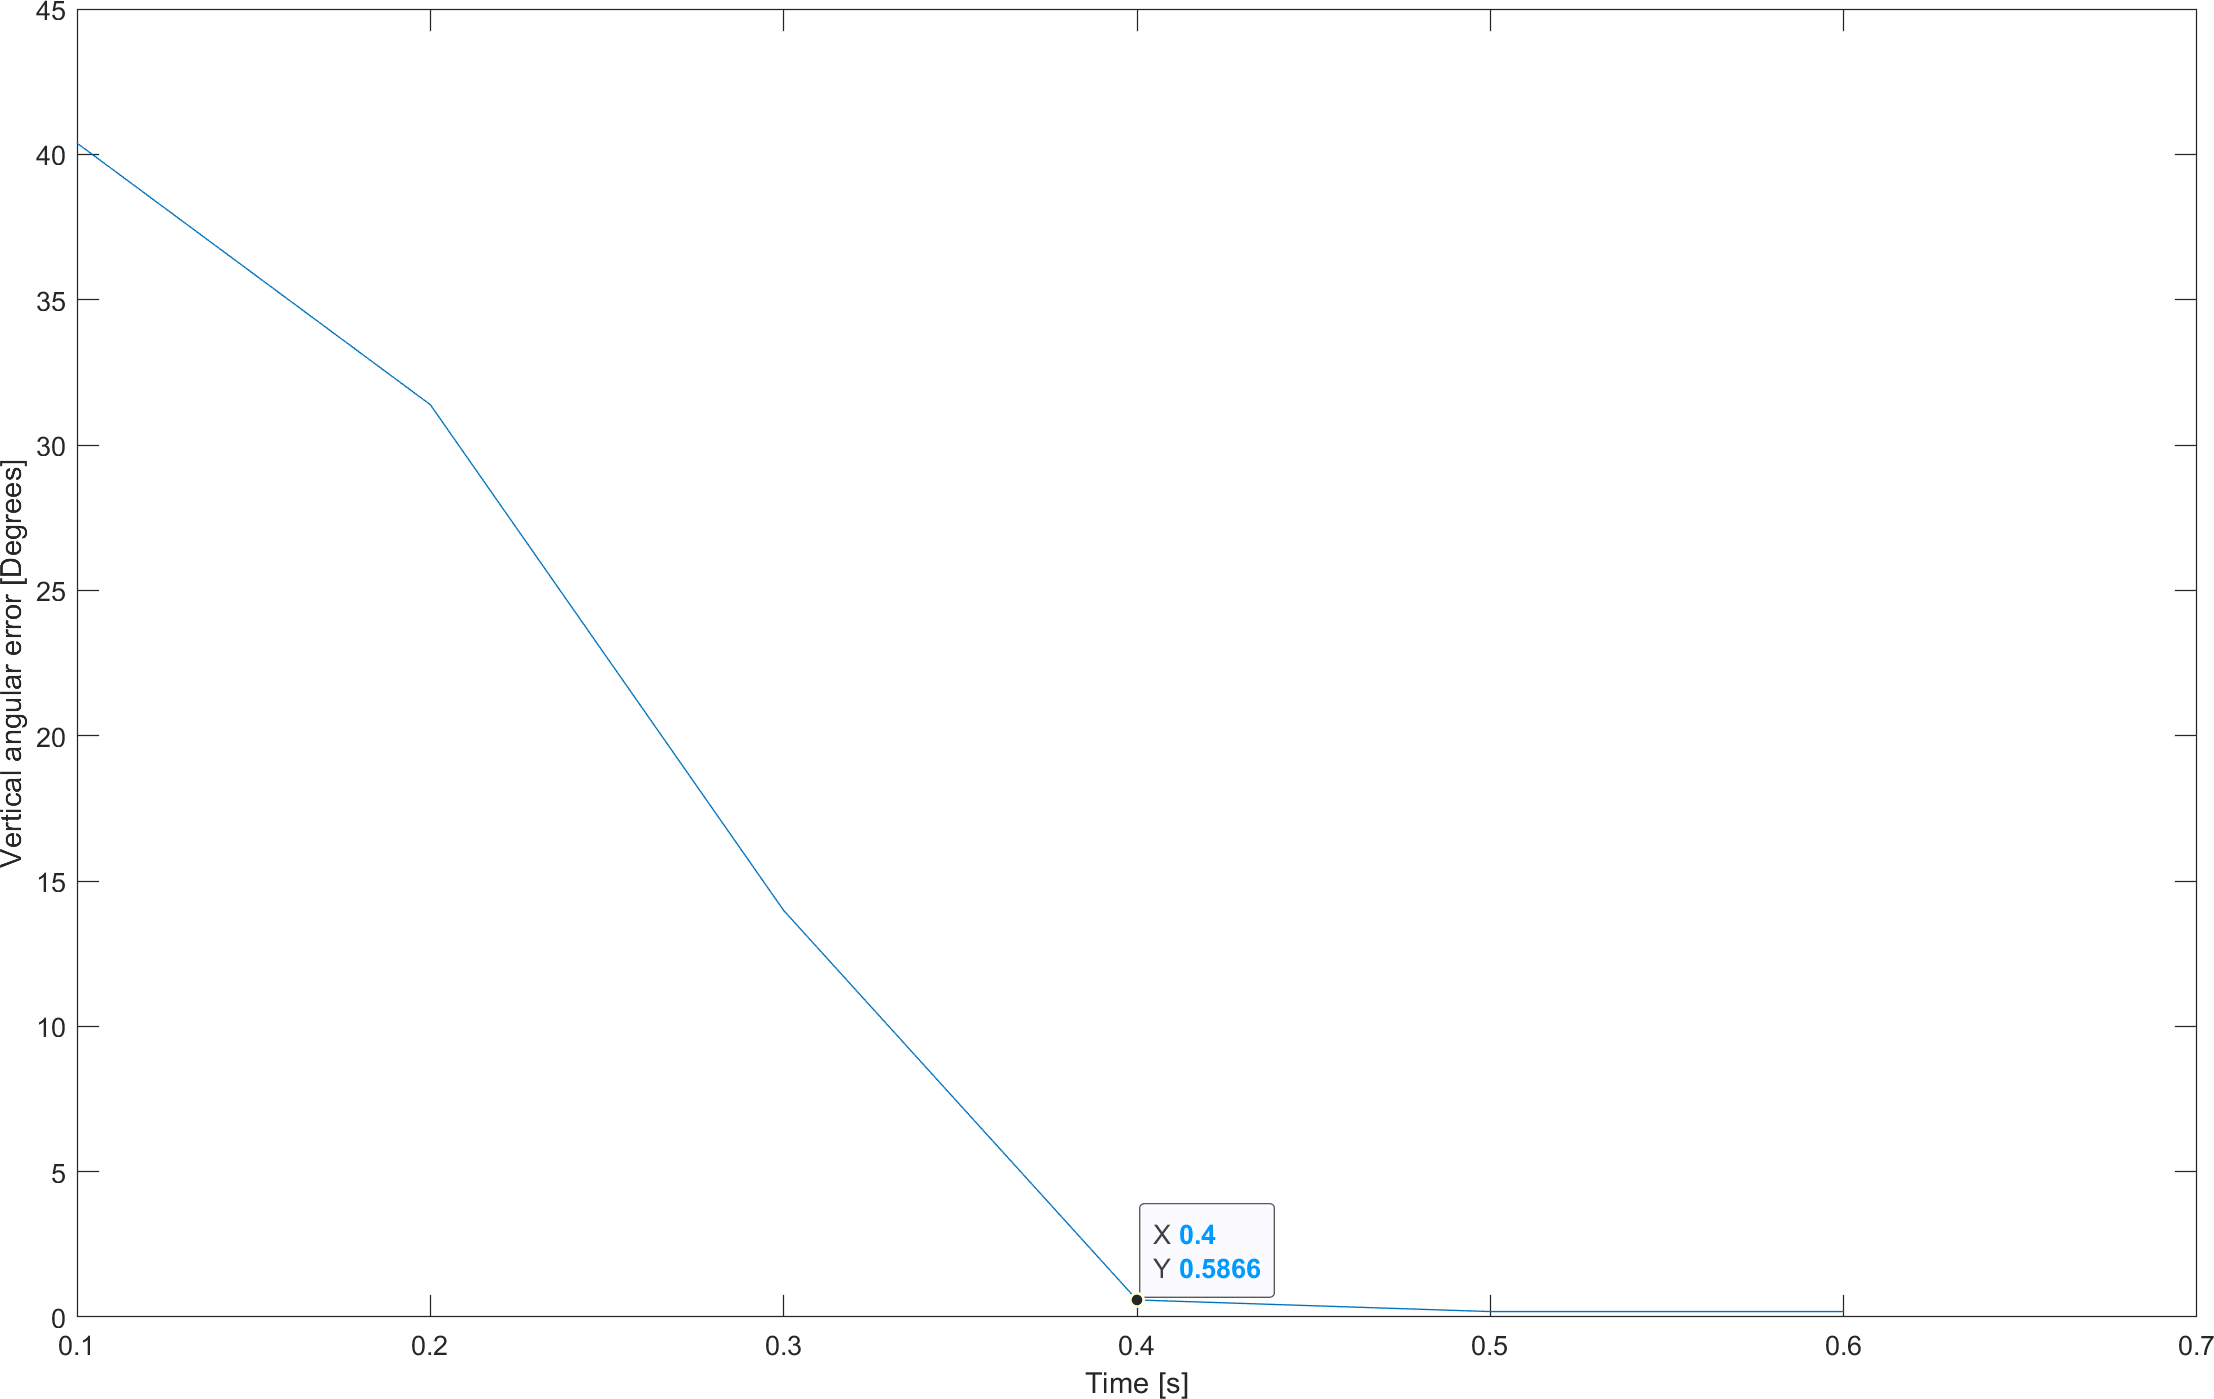
\includegraphics[width=\textwidth]{assets/Vertical_P_controller.png}
\caption{Evolution of vertical angular error from \(40^{\circ}\) step with P-controller.}
\label{vert_P}
\end{figure}
Both rise time and settling time of the vertical P controller is 0.4 seconds.
\begin{figure}[H]
\centering
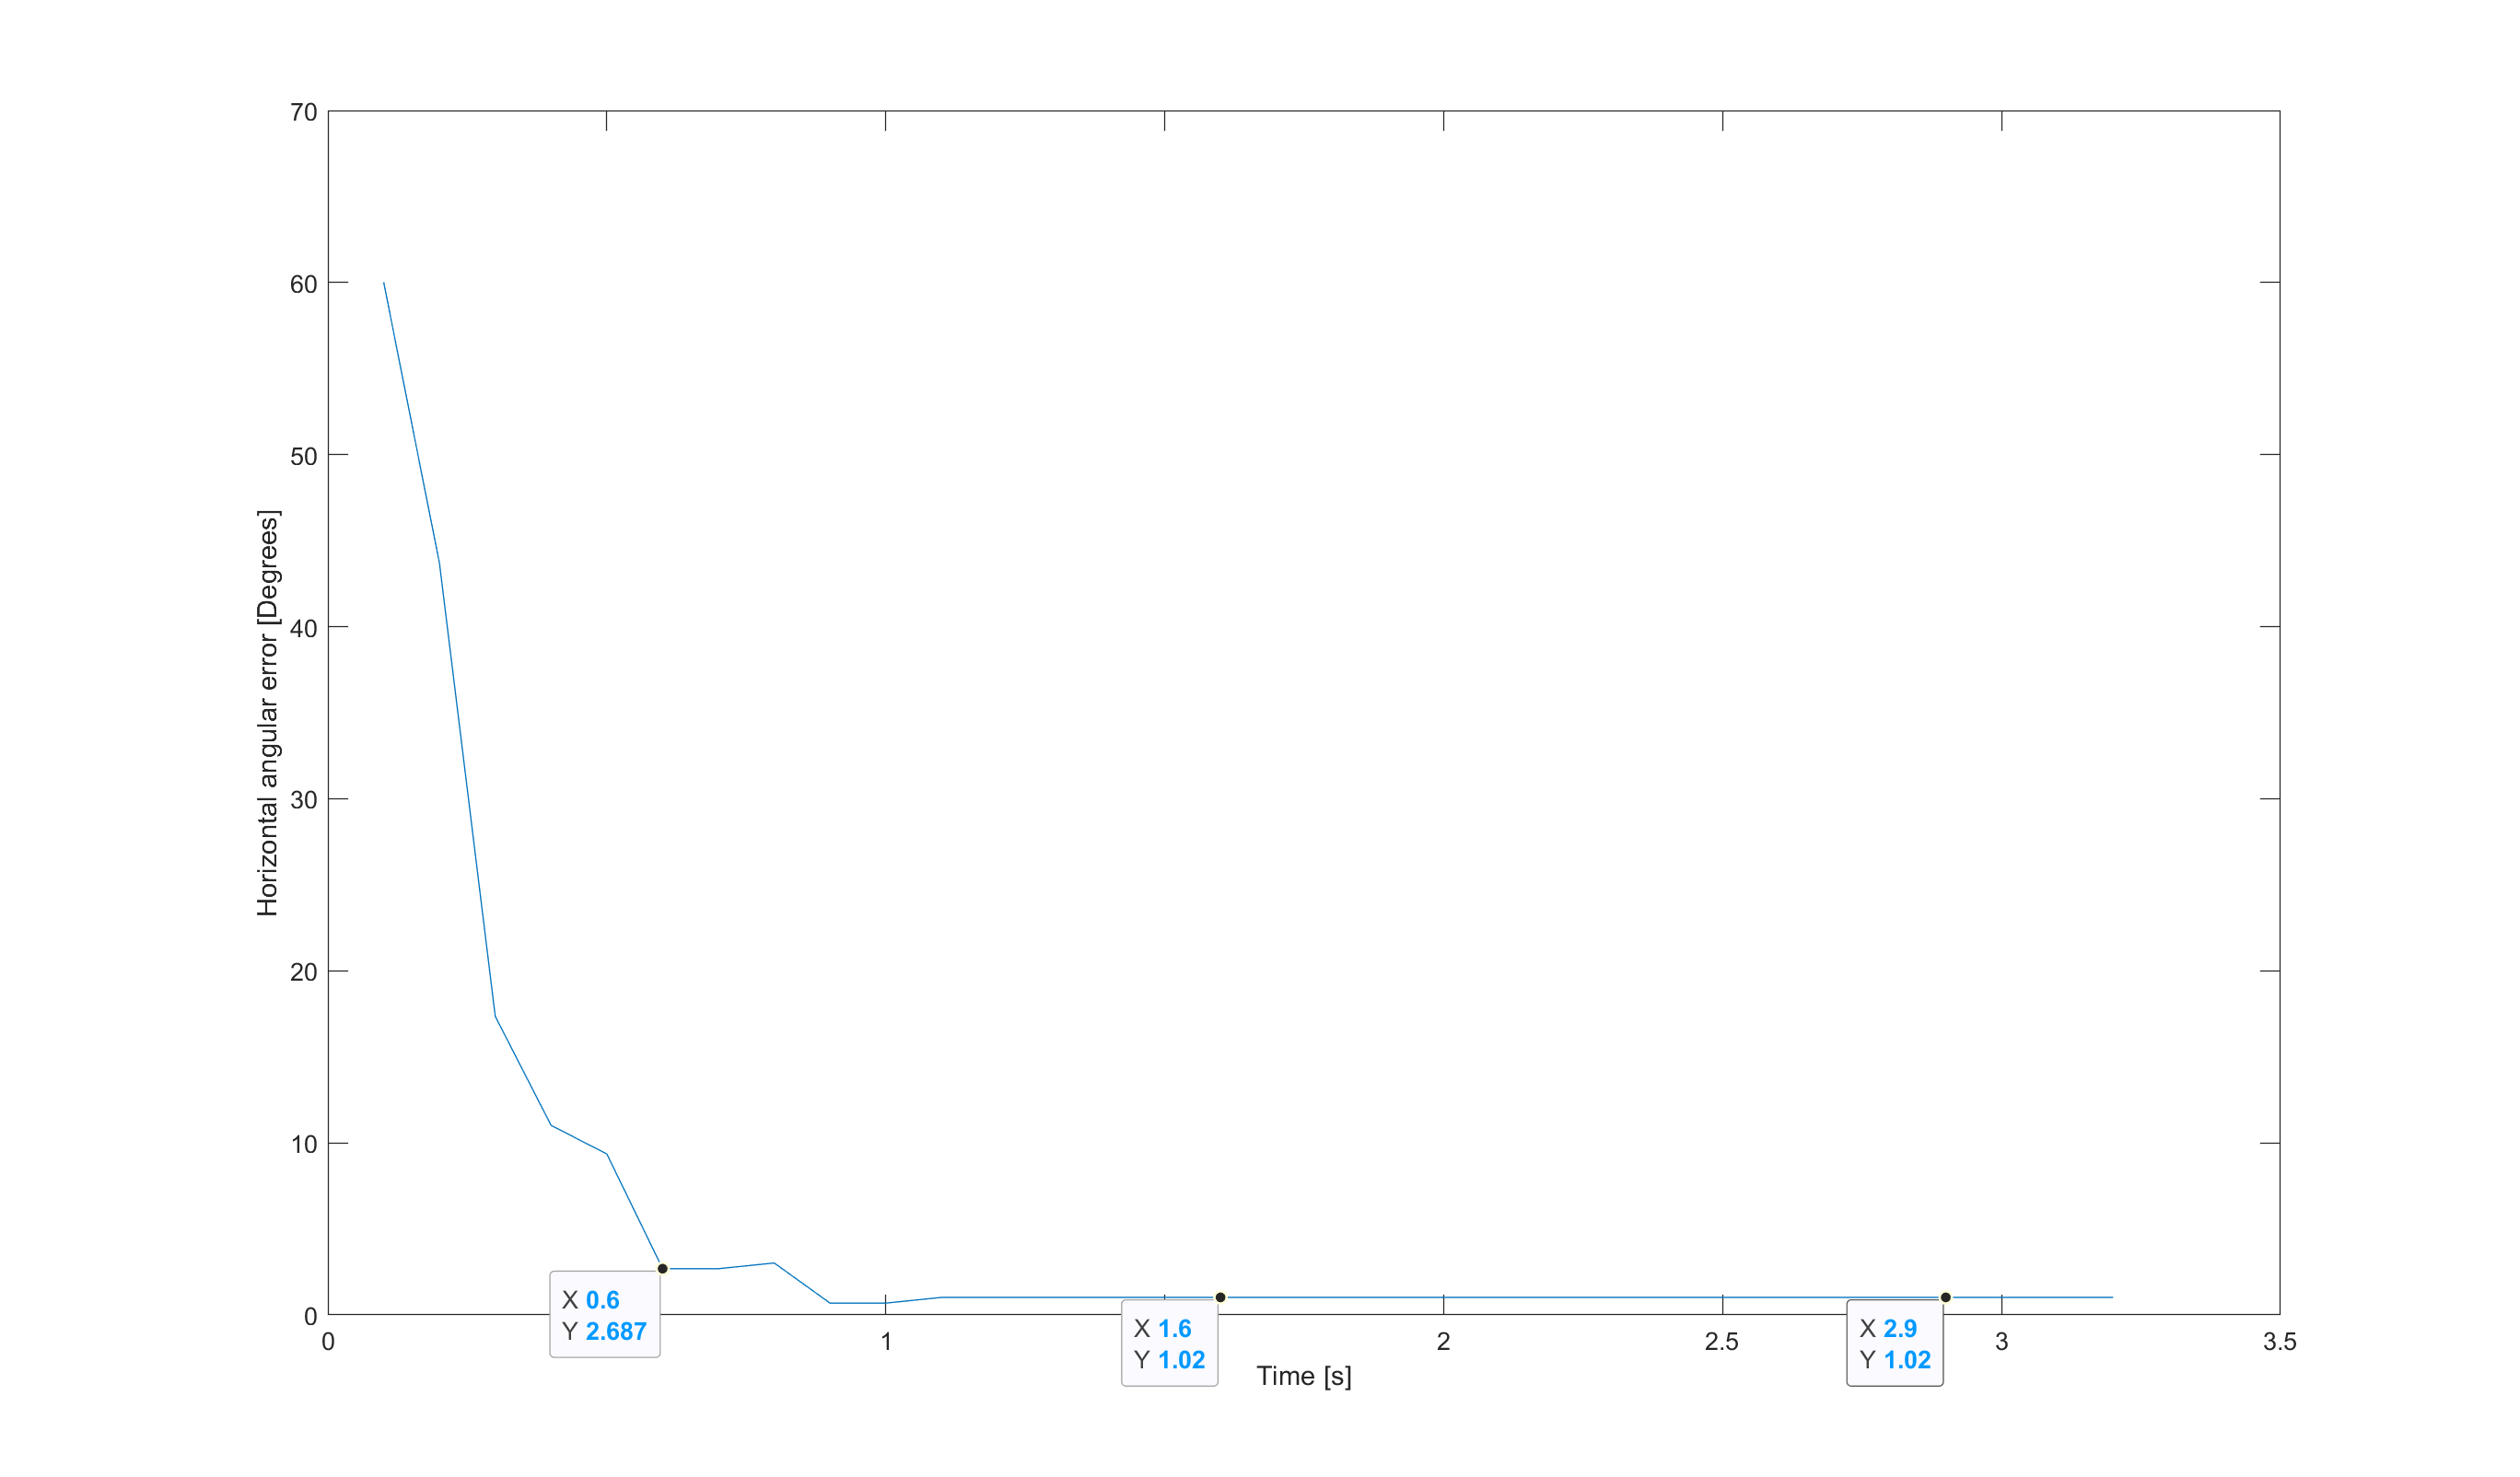
\includegraphics[width=\textwidth]{assets/Horizontal_P_controller.png}
\caption{Evolution of horizontal angular error from \(60^{\circ}\) step with P-controller.}
\label{vert_P}
\end{figure}
Rise time of horizontal P controller is 0.6 seconds and settling time is 1.6 seconds

\subsubsection{PI controllers}
\begin{figure}[H]
\centering
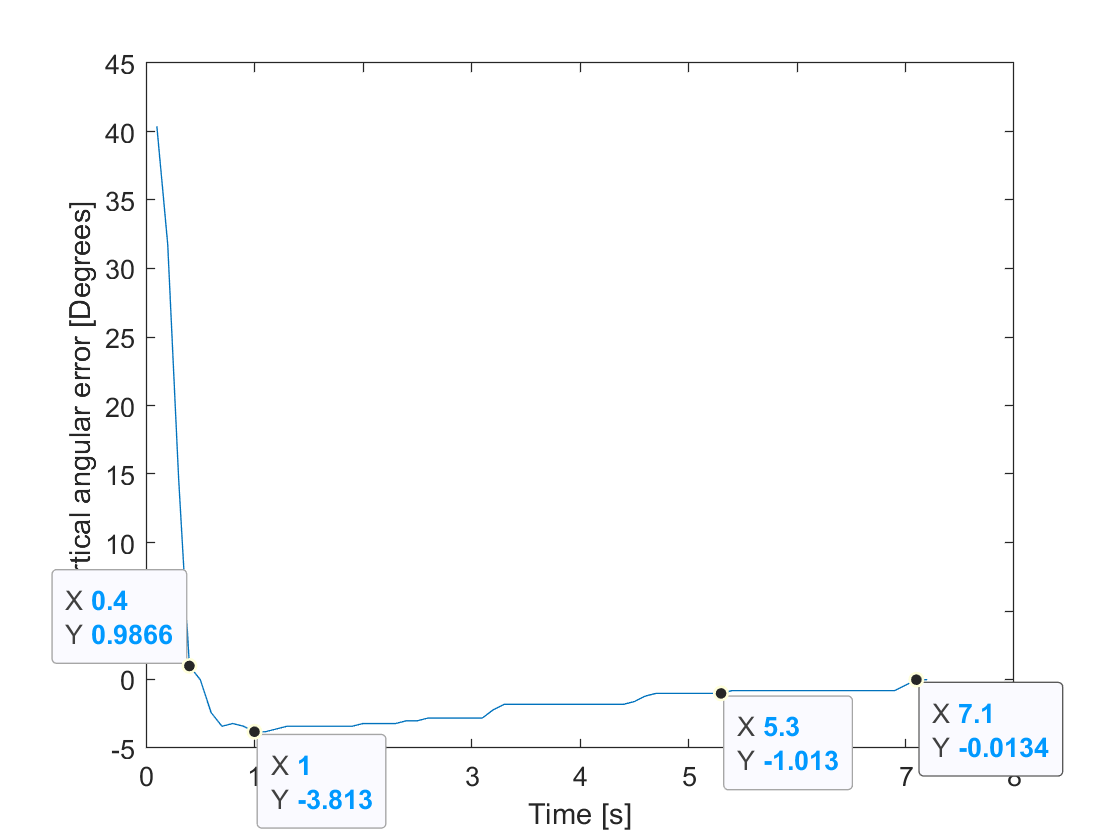
\includegraphics[width=\textwidth]{assets/Vertical_PI_controller.png}
\caption{Evolution of vertical angular error from \(40^{\circ}\) step with PI-controller.}
\label{vert_P}
\end{figure}
The rise time of the vertical PI controller is 0.4 seconds and the settling time is 7.1 seconds.
\begin{figure}[H]
\centering
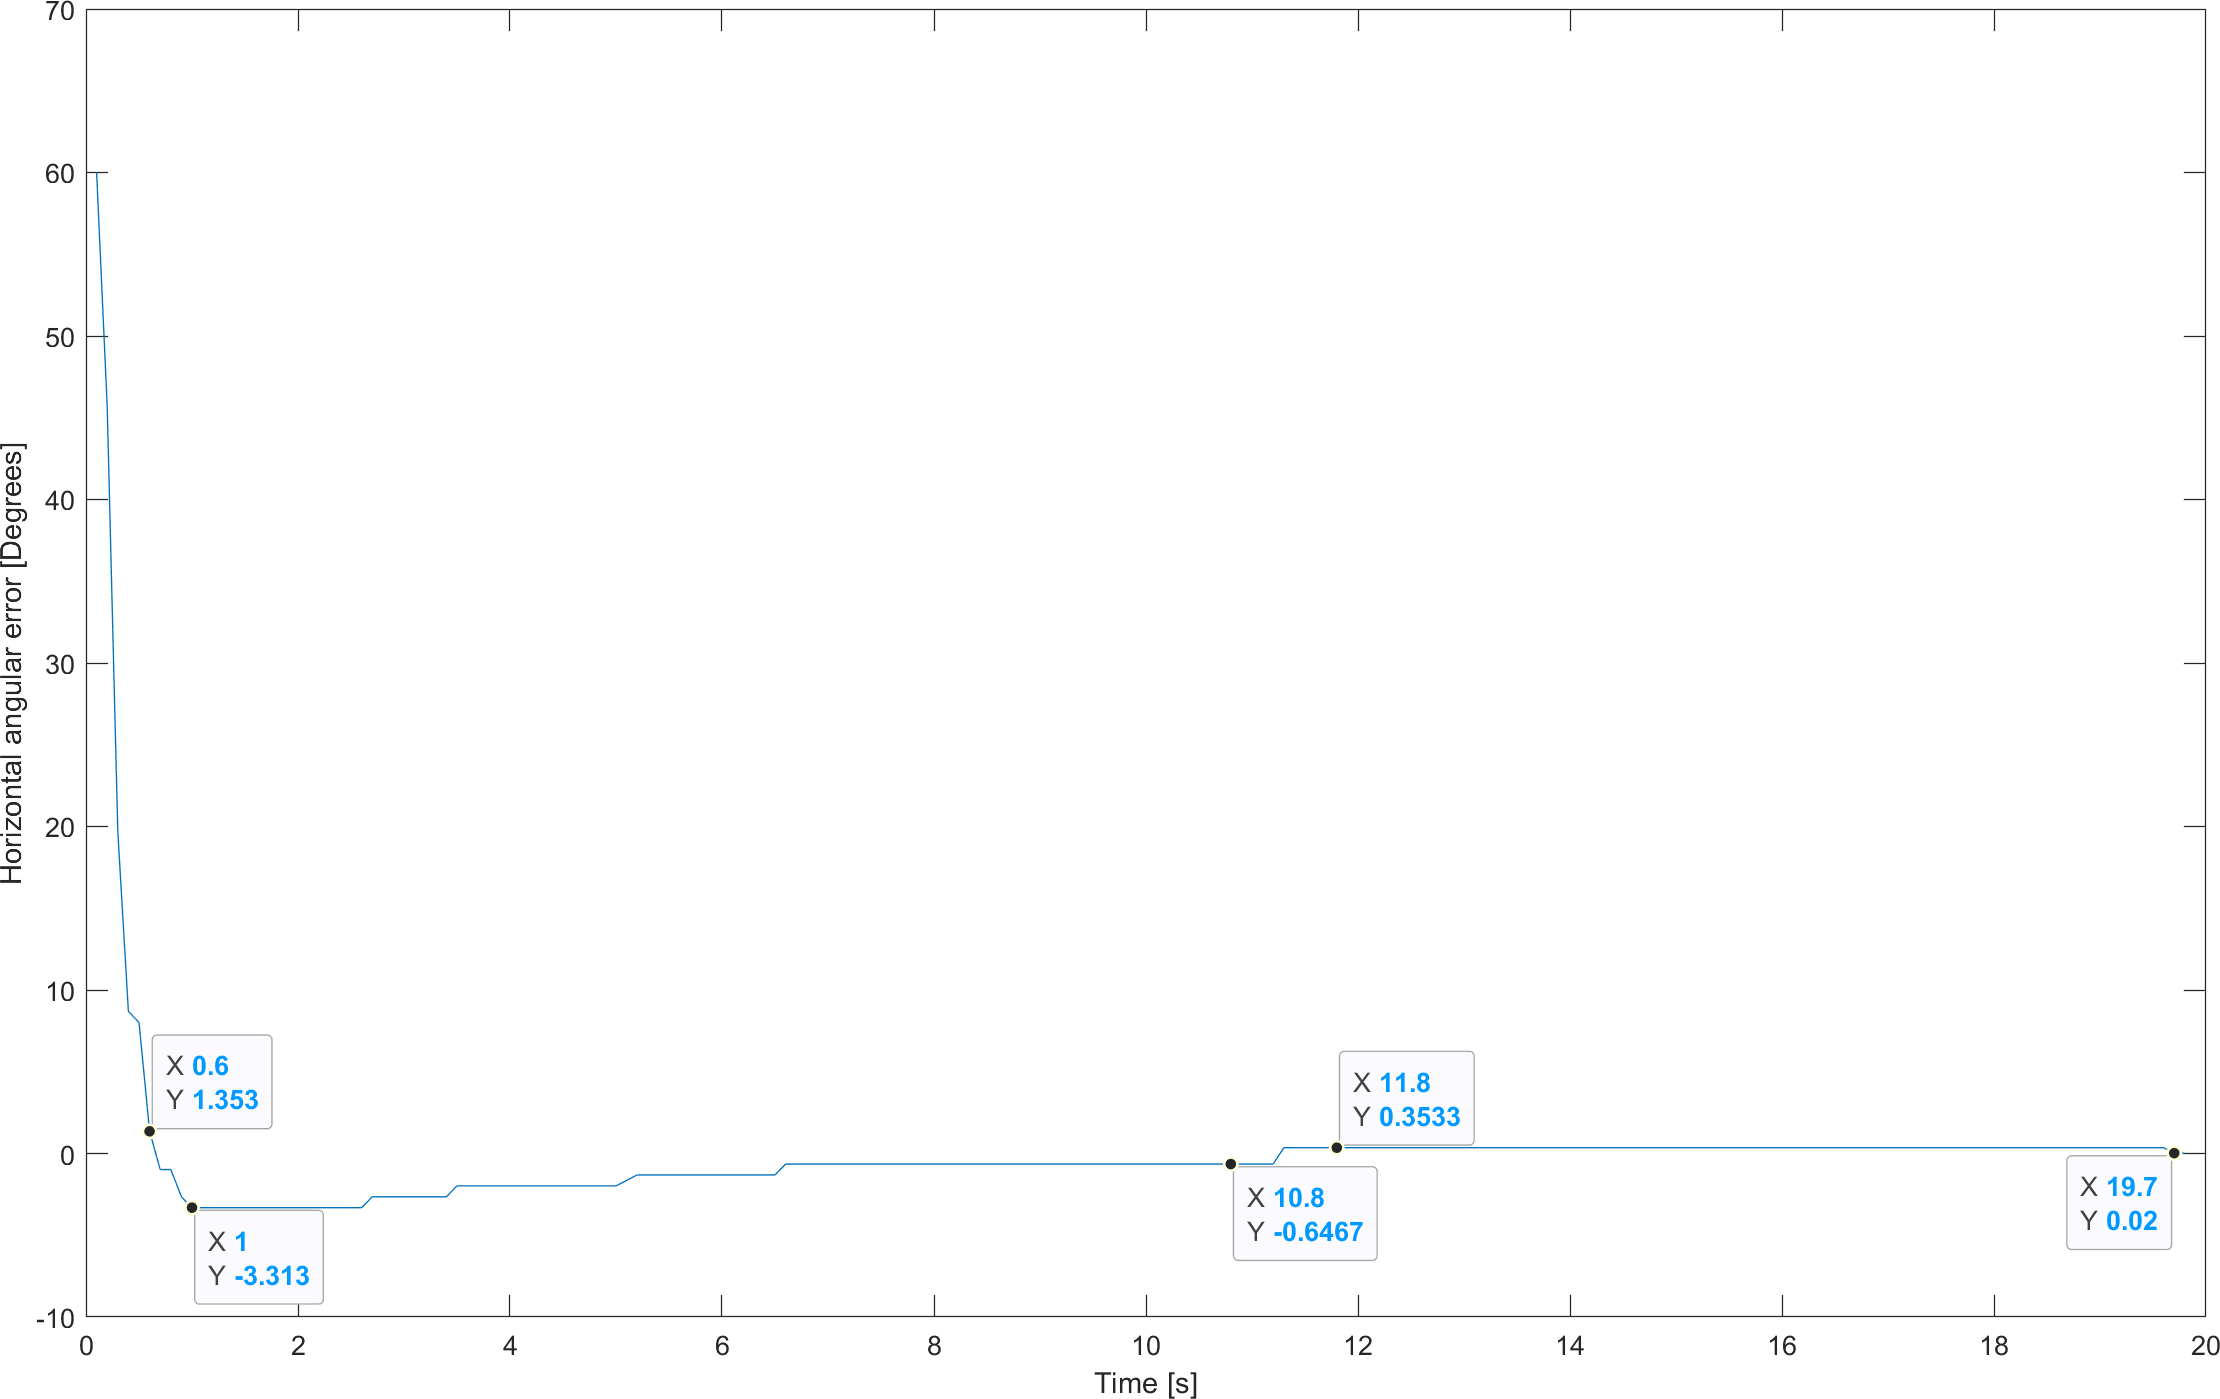
\includegraphics[width=\textwidth]{assets/Horizontal_PI_controller.png}
\caption{Evolution of horizontal angular error from \(60^{\circ}\) step with PI-controller.}
\label{vert_P}
\end{figure}
Rise time of horizontal PI controller is 0.6 seconds and settling time is 10.8 seconds.

\subsubsection{PD controllers}
\begin{figure}[H]
\centering
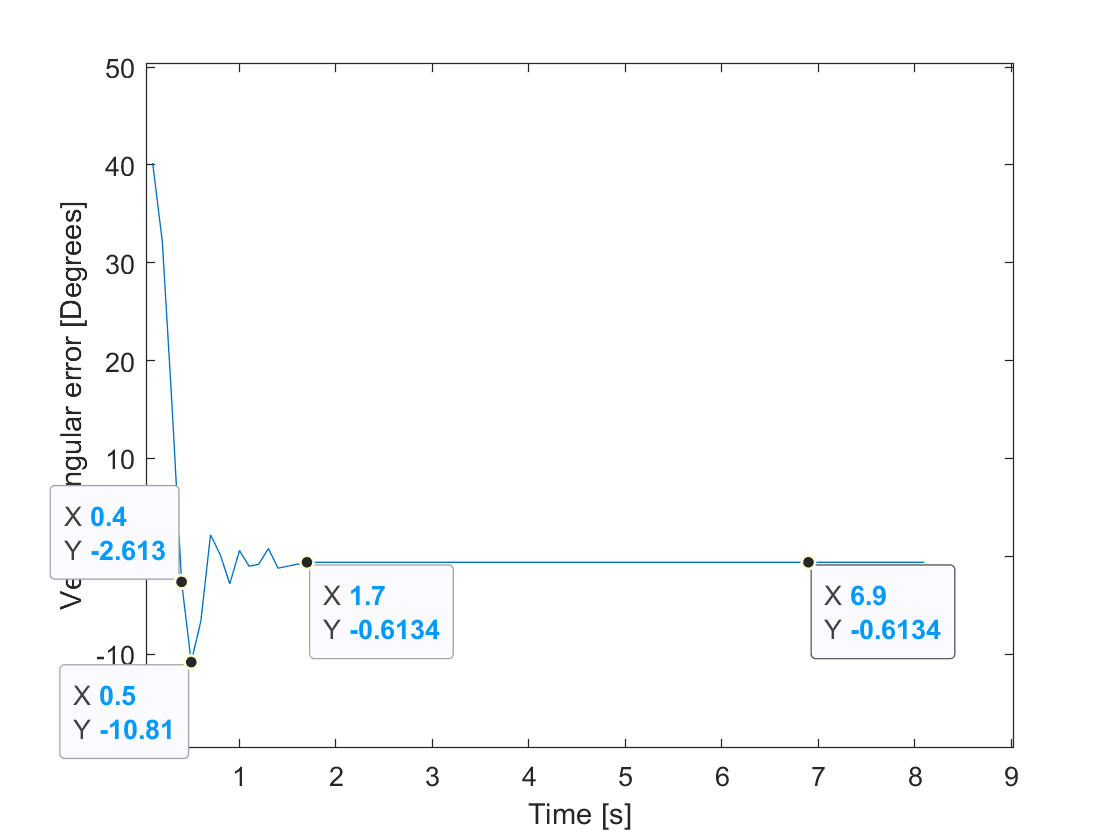
\includegraphics[width=\textwidth]{assets/Vertical_PD_controller.png}
\caption{Evolution of vertical angular error from \(40^{\circ}\) step with PD-controller.}
\label{vert_P}
\end{figure}
The rise time of the vertical PD controller is 0.4 seconds and the settling time is 1.7 seconds.
\begin{figure}[H]
\centering
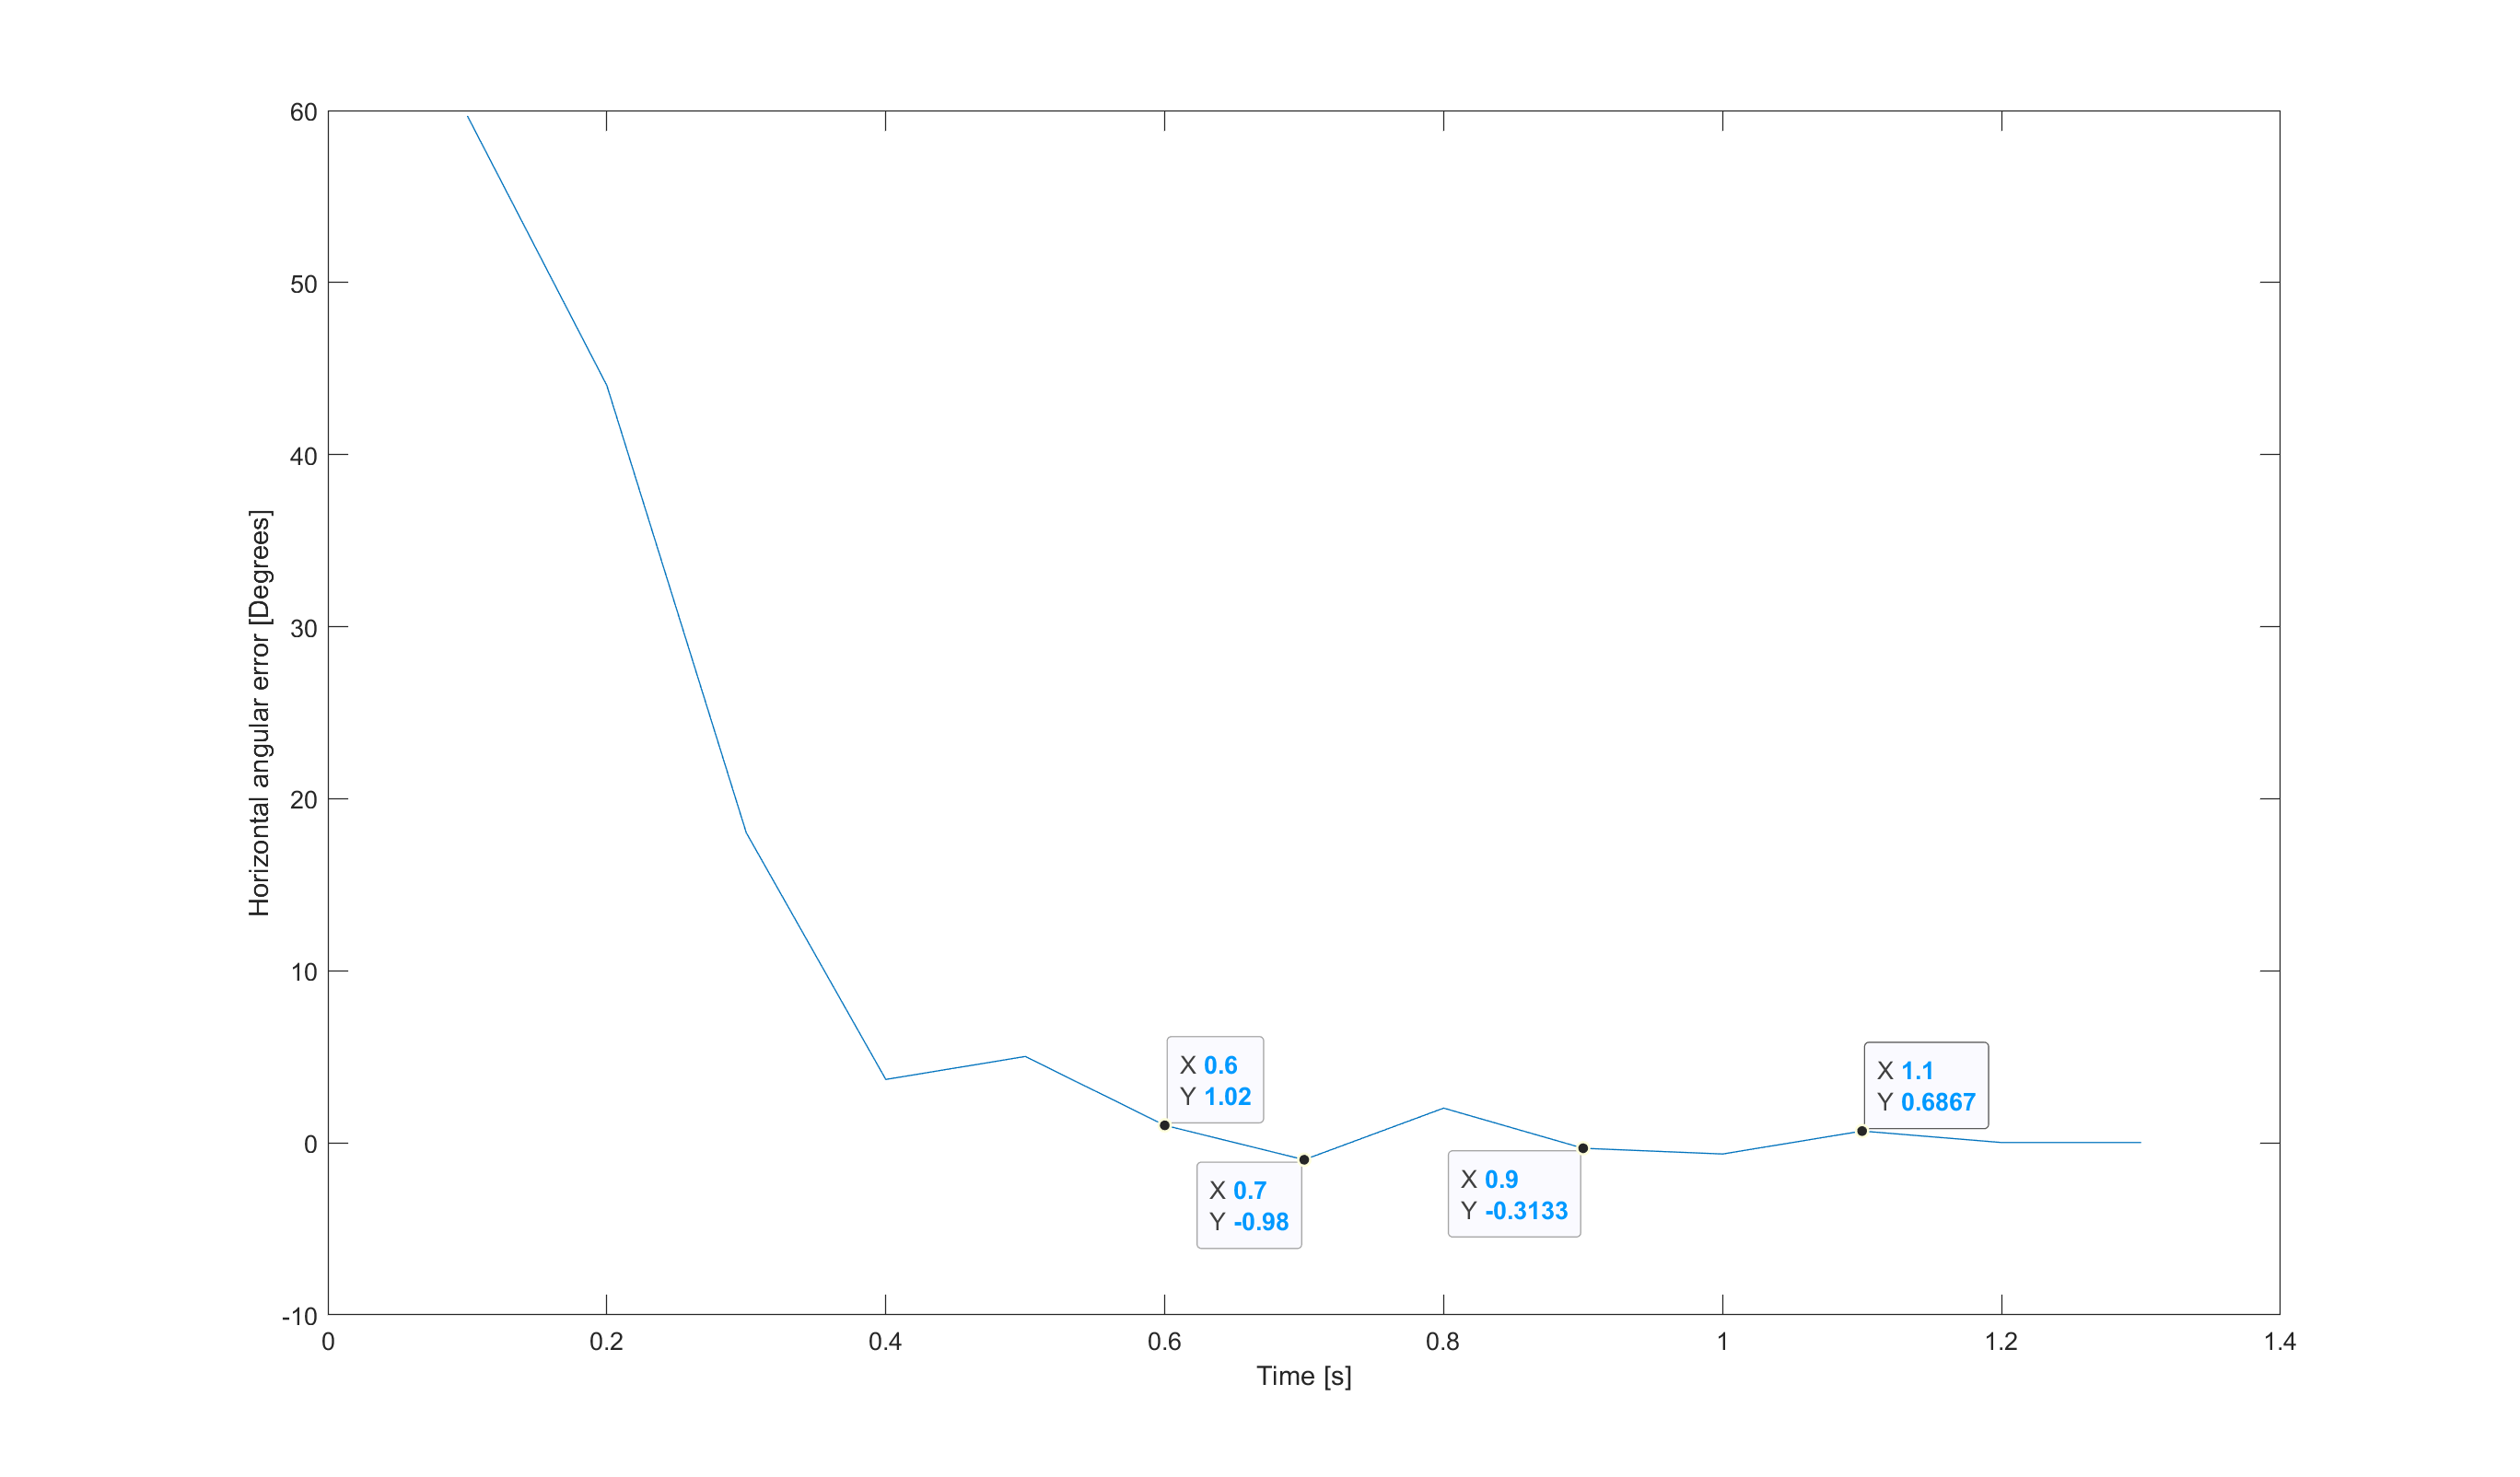
\includegraphics[width=\textwidth]{assets/Horizontal_PD_controller.png}
\caption{Evolution of horizontal angular error from \(60^{\circ}\) step with PD-controller.}
\label{vert_P}
\end{figure}
Rise time of horizontal PI controller is 0.6 seconds and settling time is 0.9 seconds.

\subsubsection{PID controllers}
\begin{figure}[H]
\centering
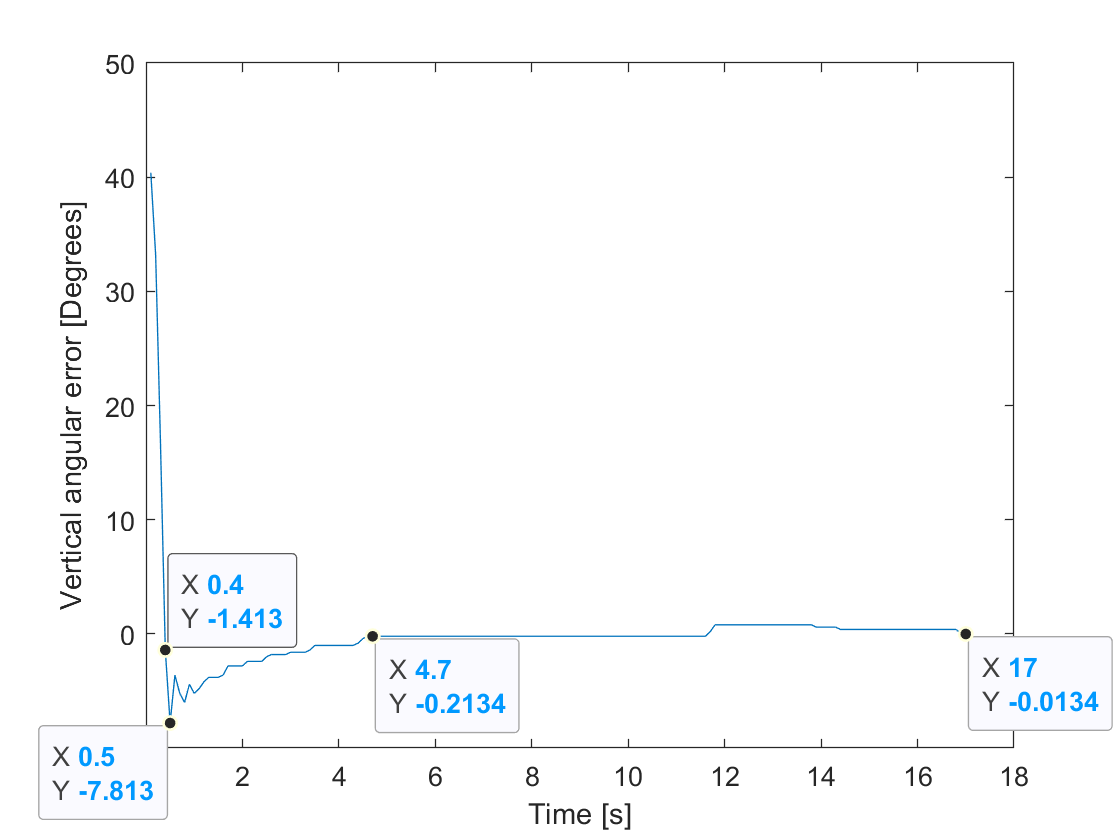
\includegraphics[width=\textwidth]{assets/Vertical_PID_controller.png}
\caption{Evolution of vertical angular error from \(40^{\circ}\) step with PID-controller.}
\label{vert_P}
\end{figure}
The rise time of the vertical PD controller is between 0.4 and 0.5 seconds and the settling time is 4.7 seconds.
\begin{figure}[H]
\centering
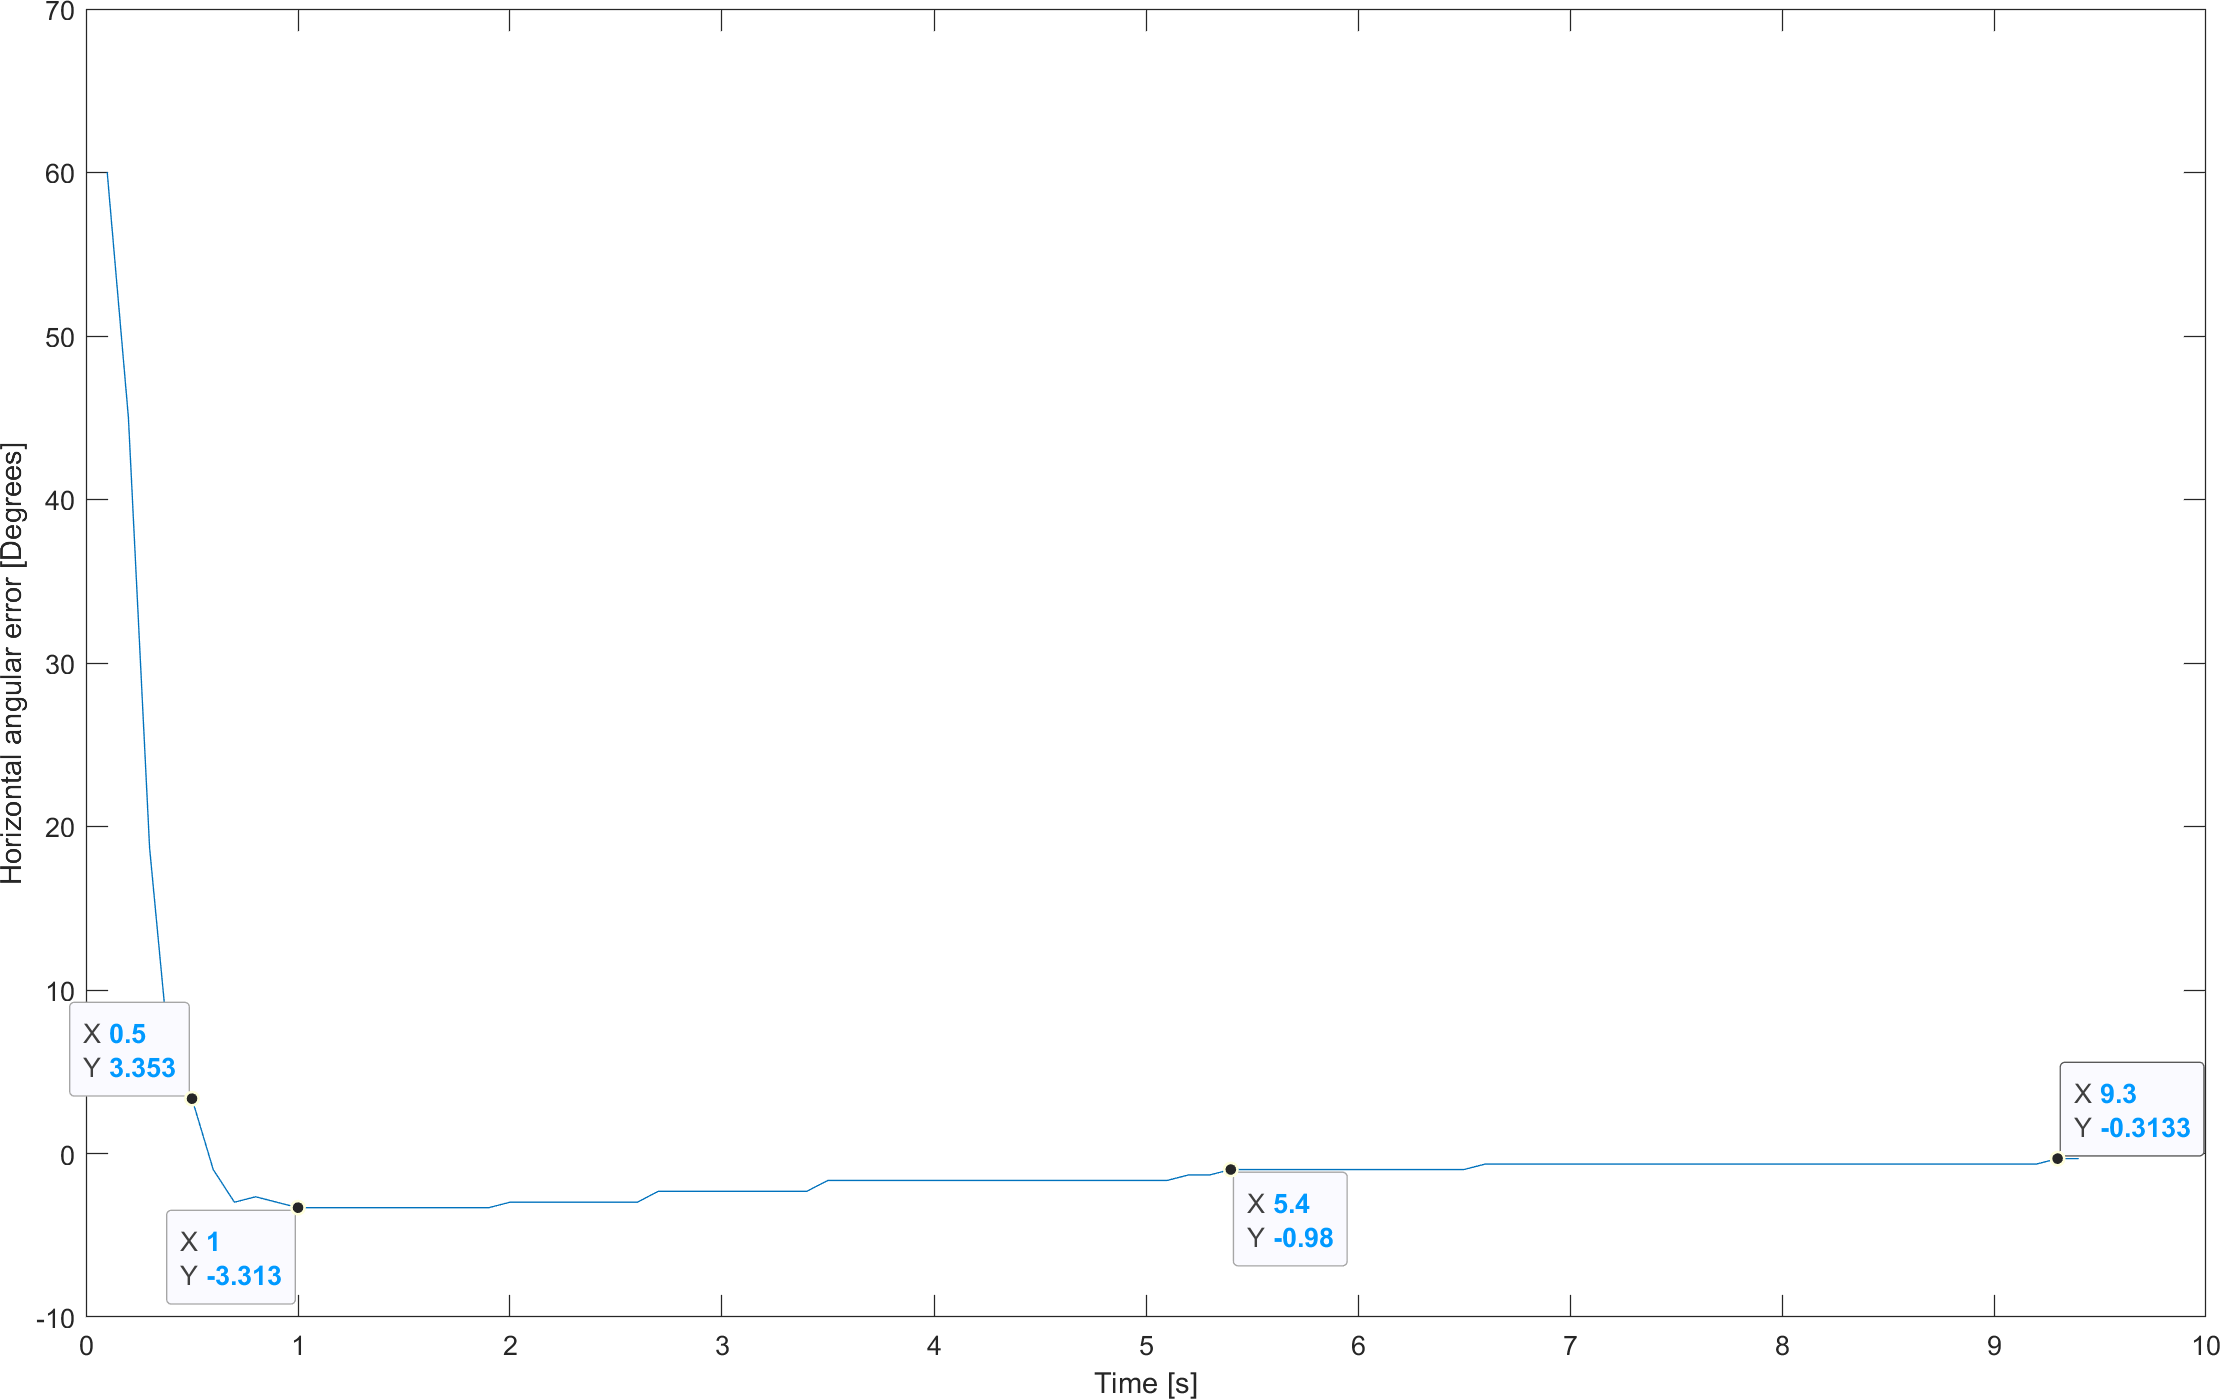
\includegraphics[width=\textwidth]{assets/Horizontal_PID_controller.png}
\caption{Evolution of horizontal angular error from \(60^{\circ}\) step with PID-controller.}
\label{vert_P}
\end{figure}
Rise time of horizontal PI controller is between 0.5 and 0.6 seconds and settling time is 5.4 seconds.

\subsubsection{BrickPi3 library for controlling robot arm movement}
\begin{figure}[H]
\centering
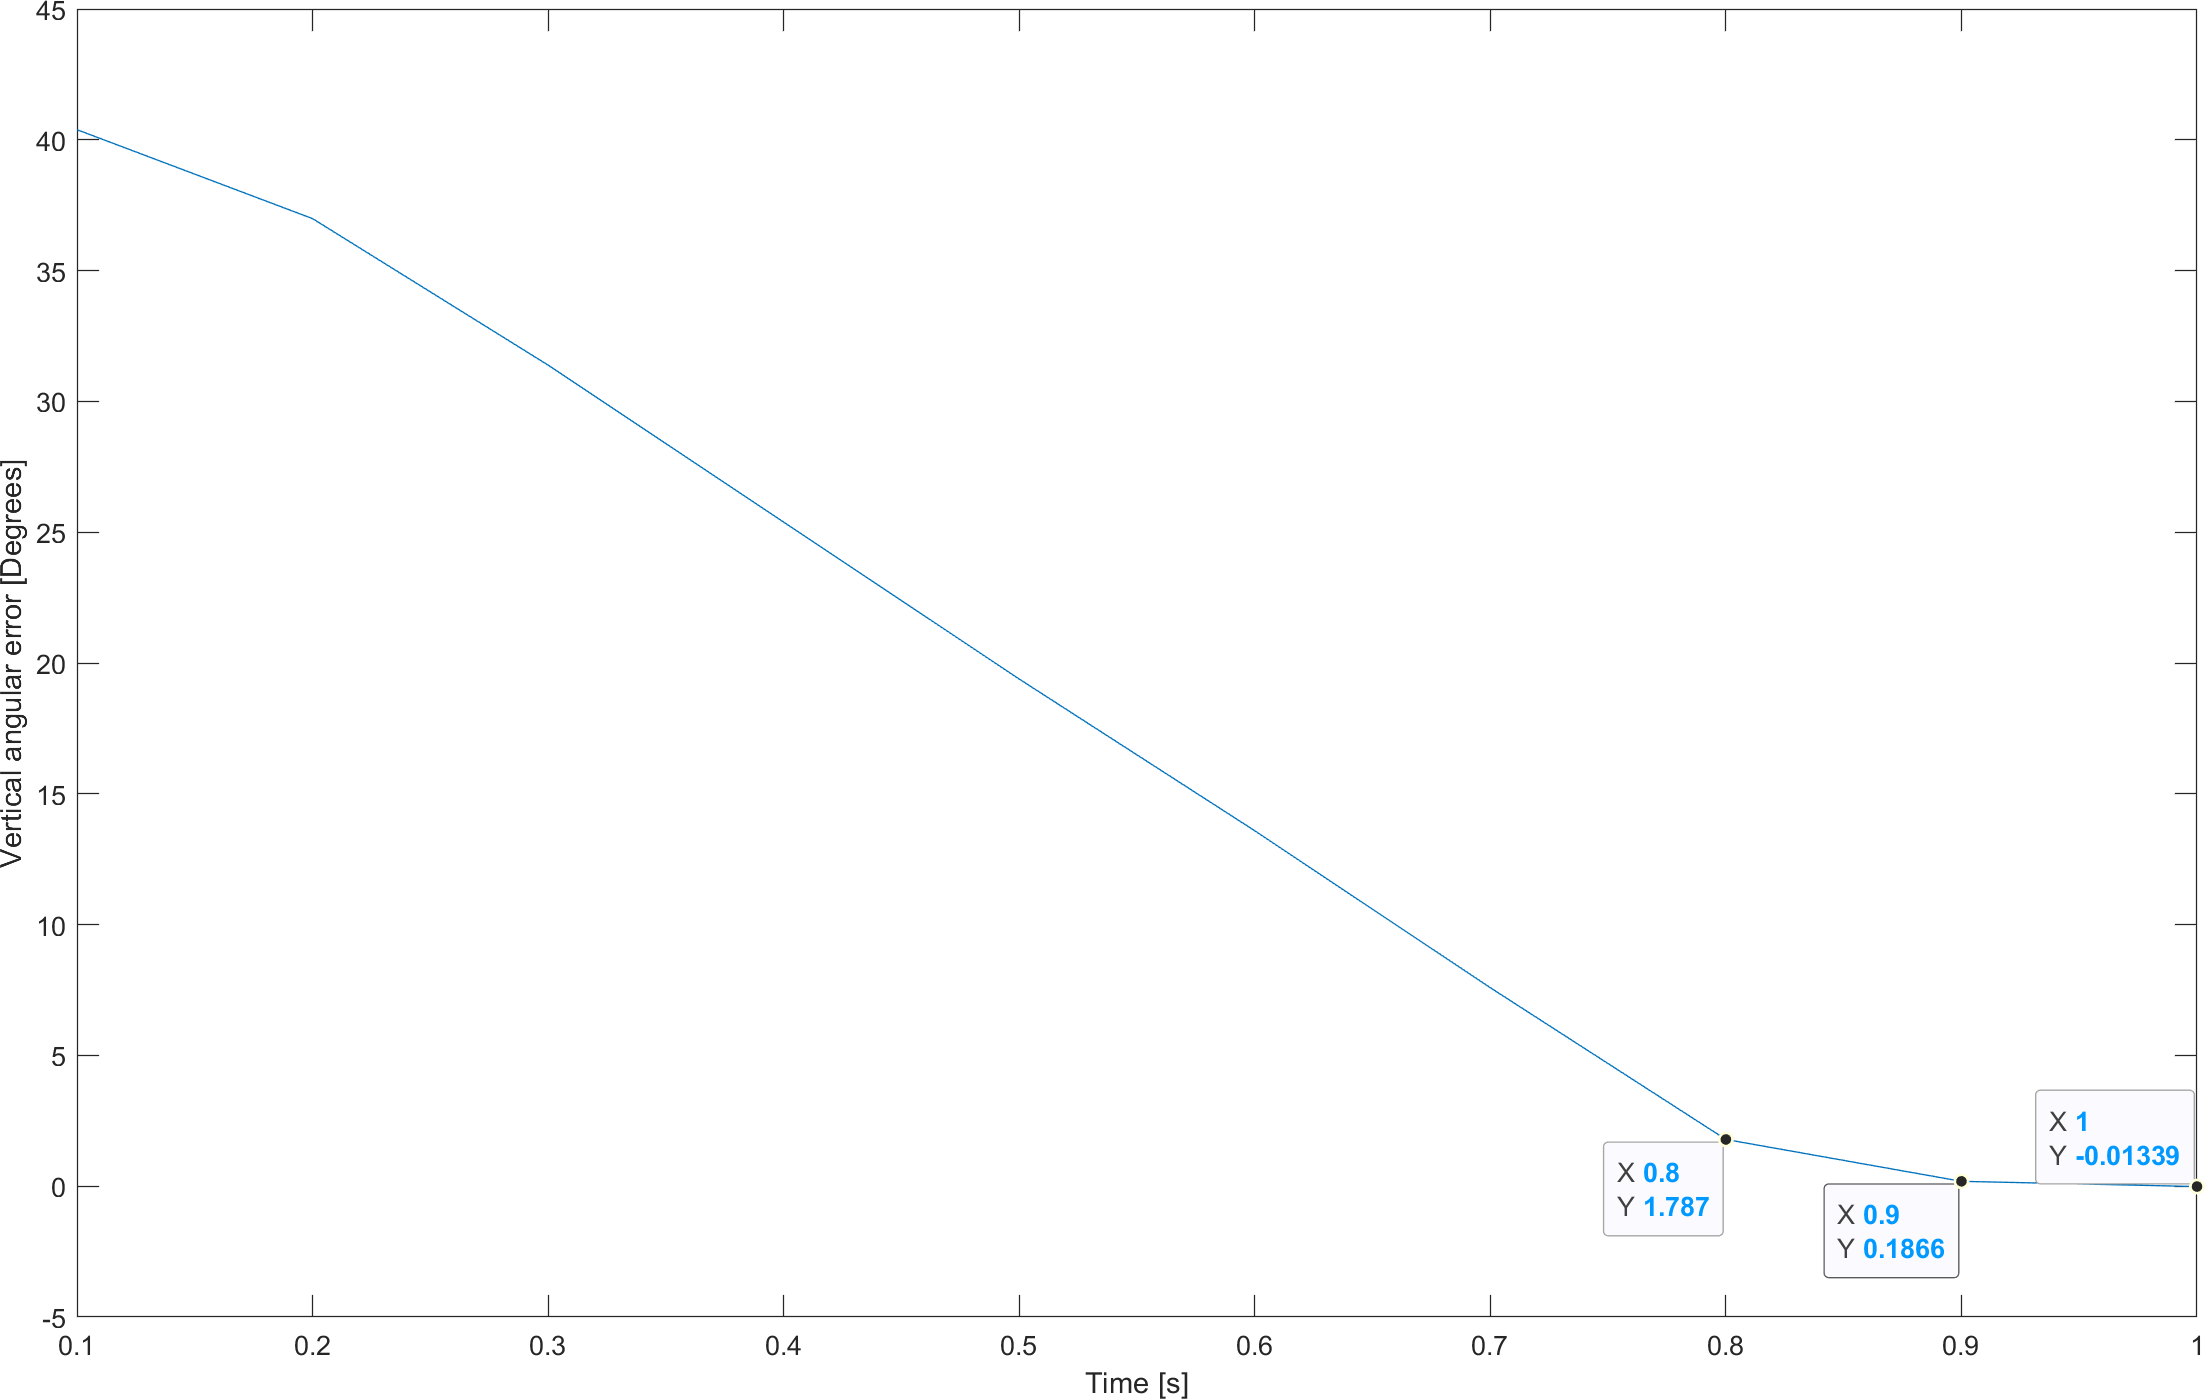
\includegraphics[width=\textwidth]{assets/Vertical_built_in_functions.png}
\caption{Evolution of vertical angular error from \(40^{\circ}\) step with BrickPi3 library motor functions.}
\label{vert_P}
\end{figure}
The rise time of the vertical PD controller is between 0.8 seconds and the settling time is 0.9 seconds.
\begin{figure}[H]
\centering
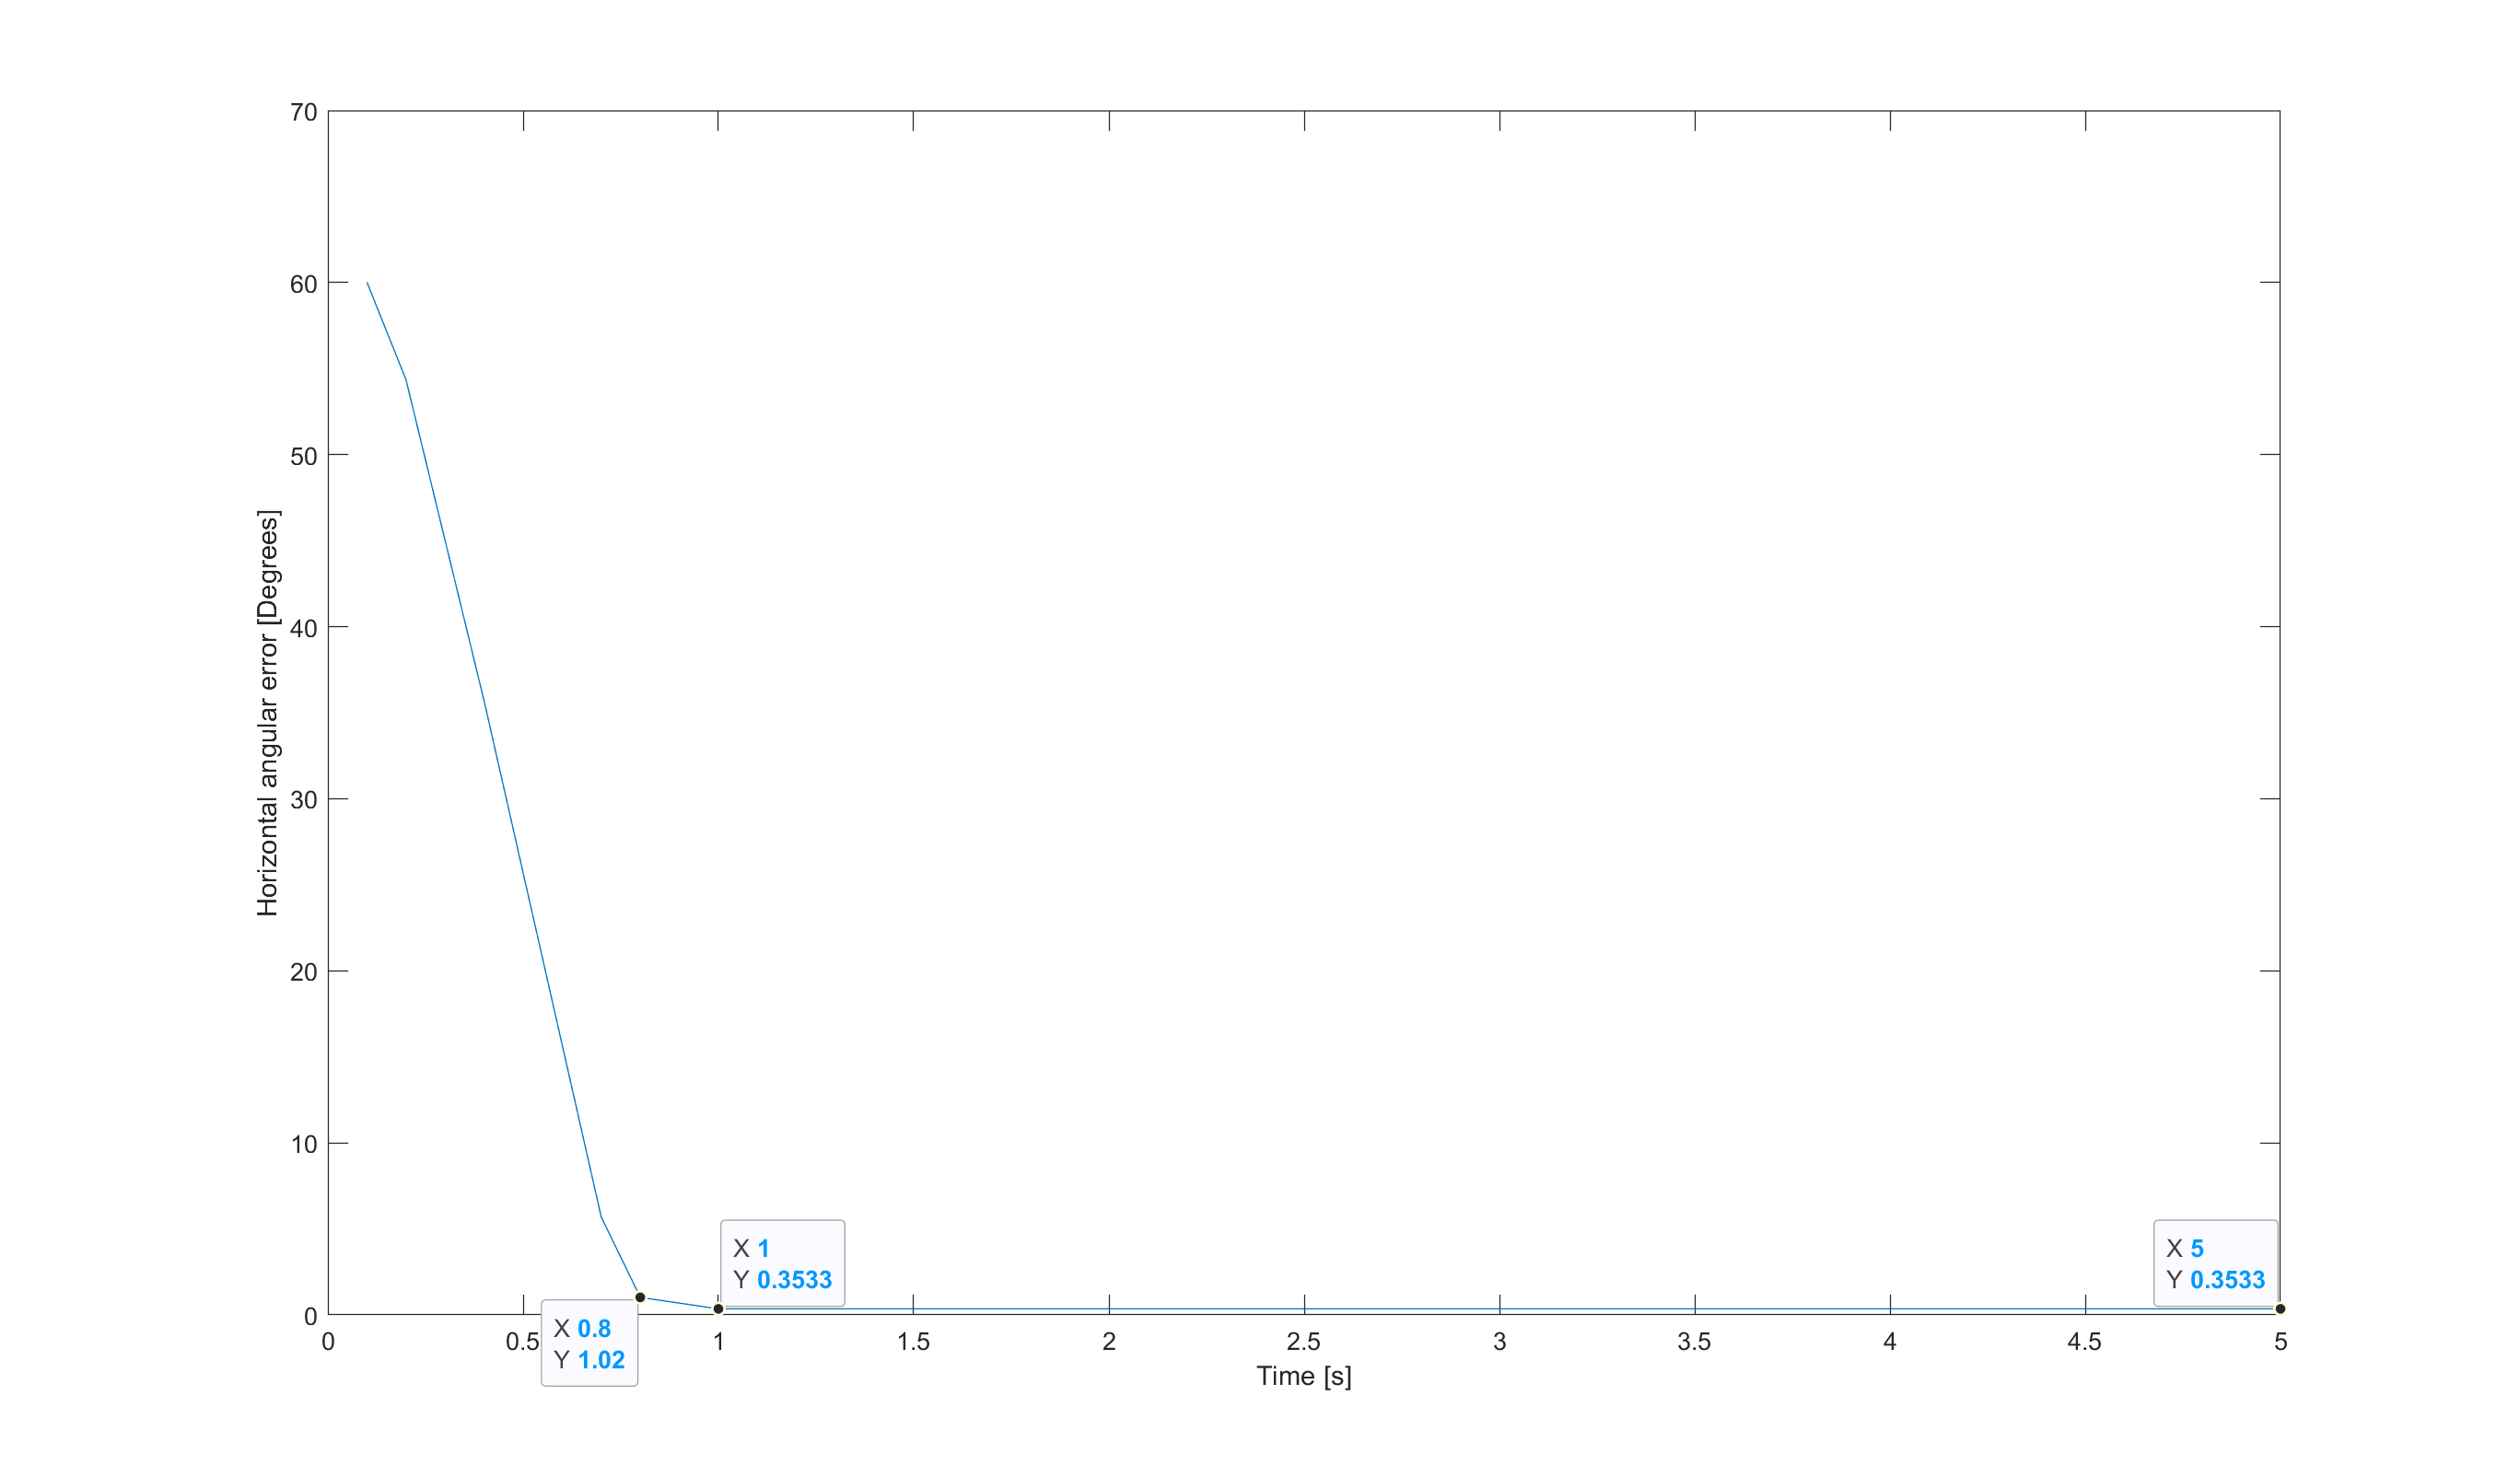
\includegraphics[width=\textwidth]{assets/Horizontal_built_in_funtion.png}
\caption{Evolution of horizontal angular error from \(60^{\circ}\) step with BrickPi3 library motor functions.}
\label{vert_P}
\end{figure}
Rise time of horizontal PI controller is between 0.8 seconds and settling time is 1 second.

\subsection{Ziegler Nichols tuning results}
The controllers mentioned above was tuned with a Ziegler Nichols approach and two plots of undamped oscillations for vertical and horizontal arm movements are shown in  Fig~\ref{vert_osc} and Fig~\ref{Hor_osc}.
\begin{figure}[H]
\centering
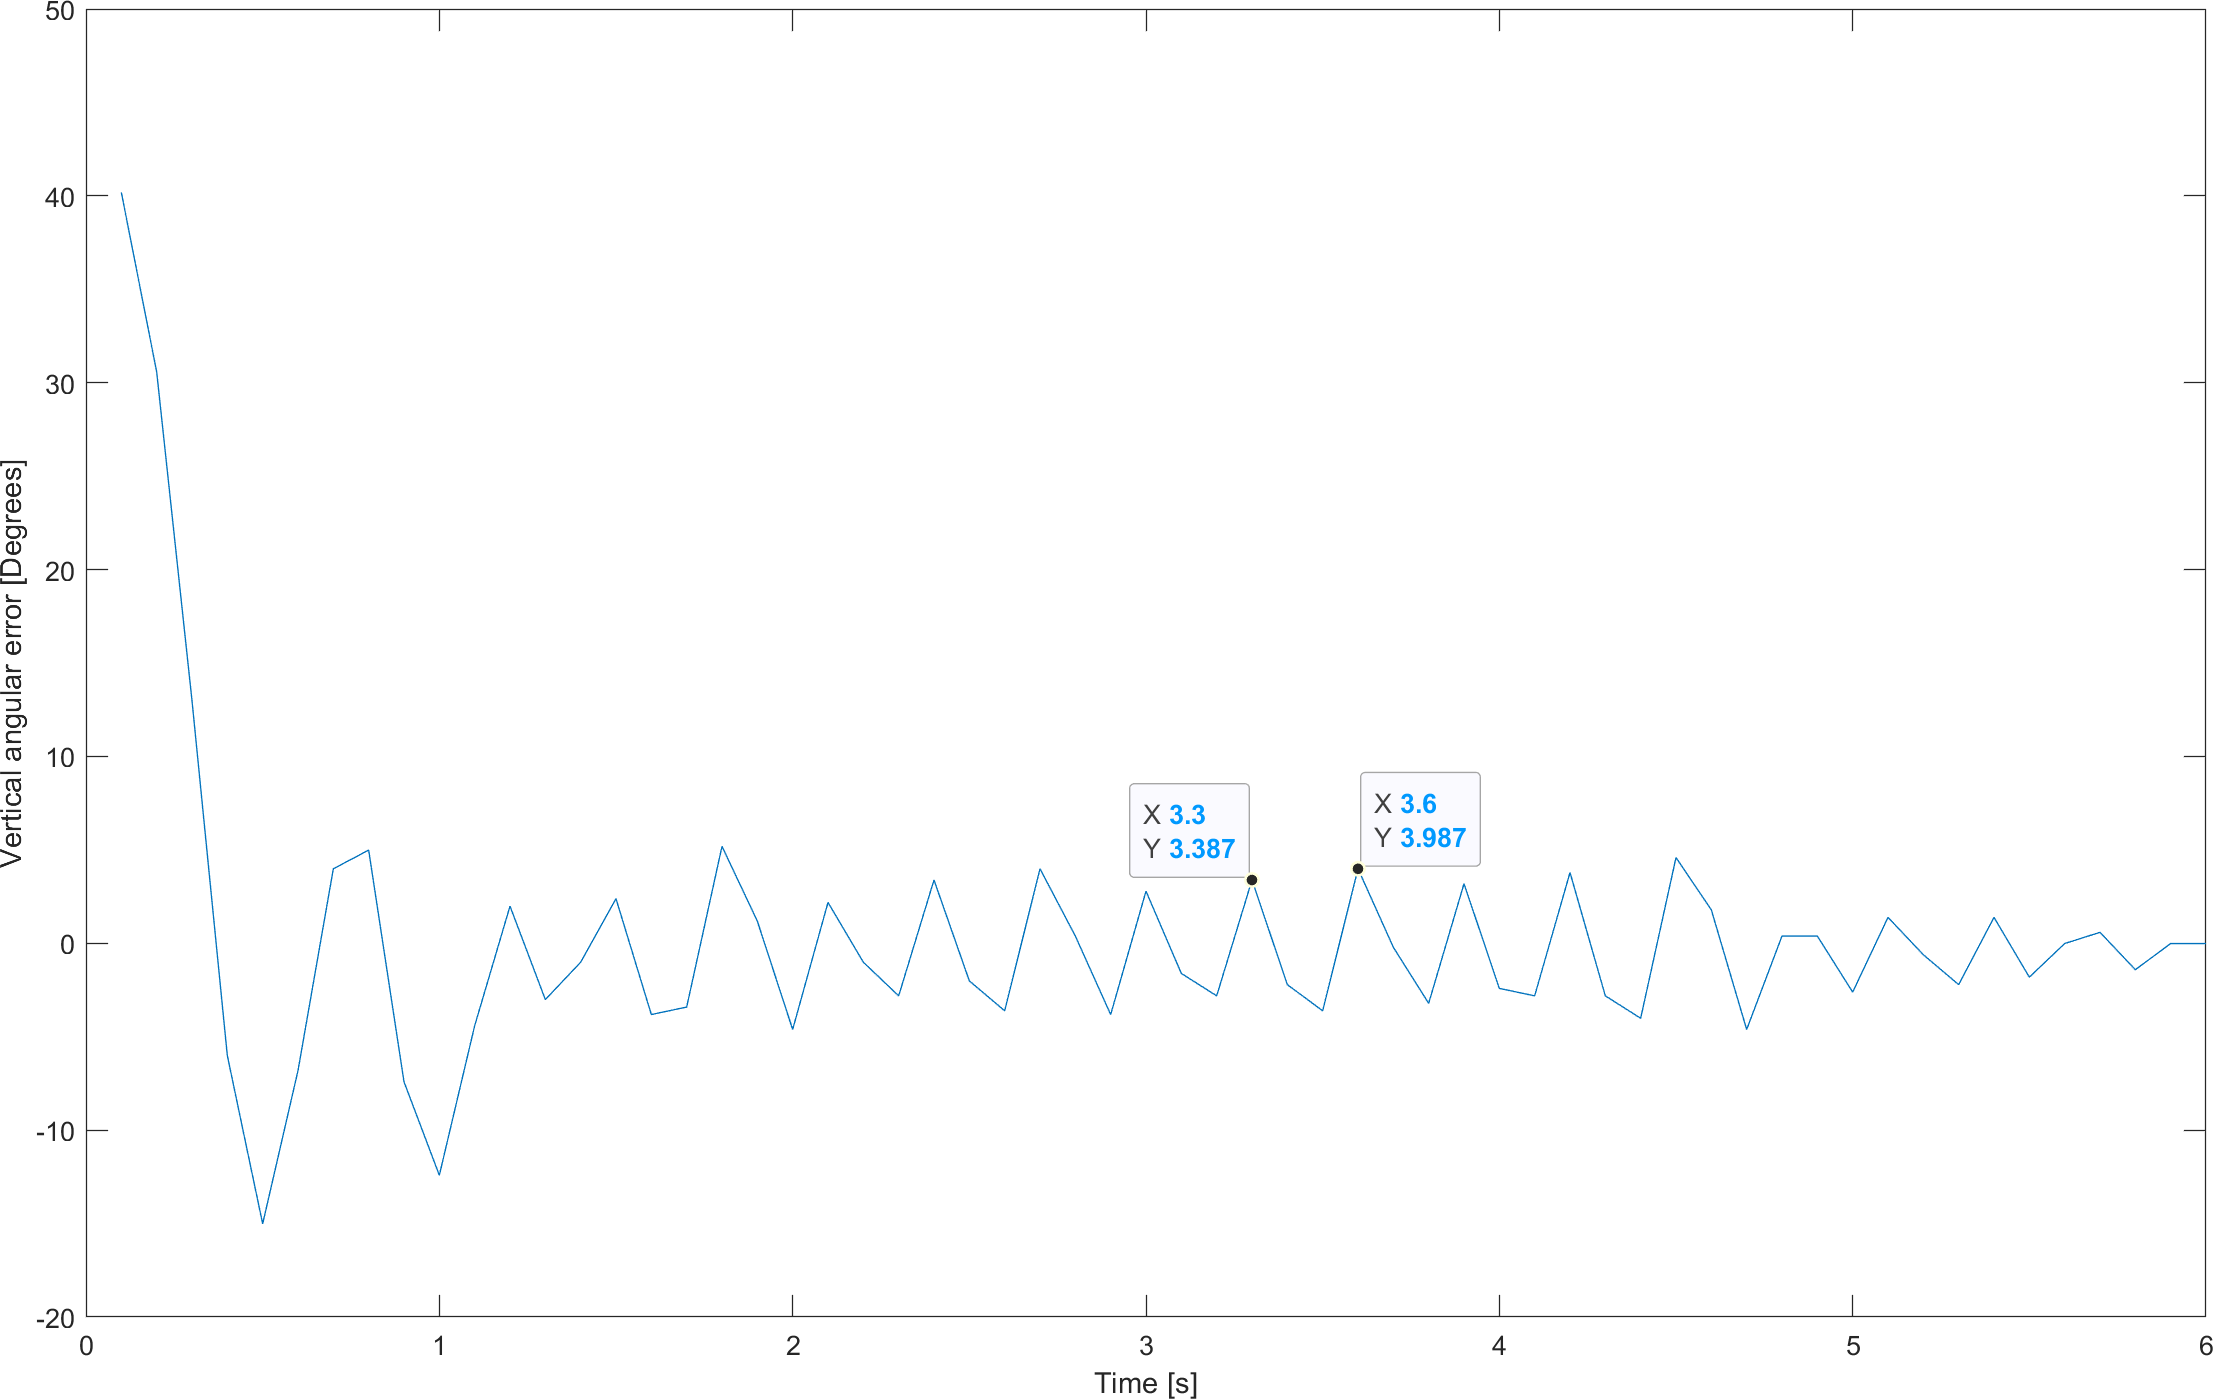
\includegraphics[width=\textwidth]{assets/Vertical_undamped_oscillation.png}
\caption{Close to undamped oscillations from \(40^{\circ}\) step with P-controller.}
\label{vert_osc}
\end{figure}
\begin{figure}[H]
\centering
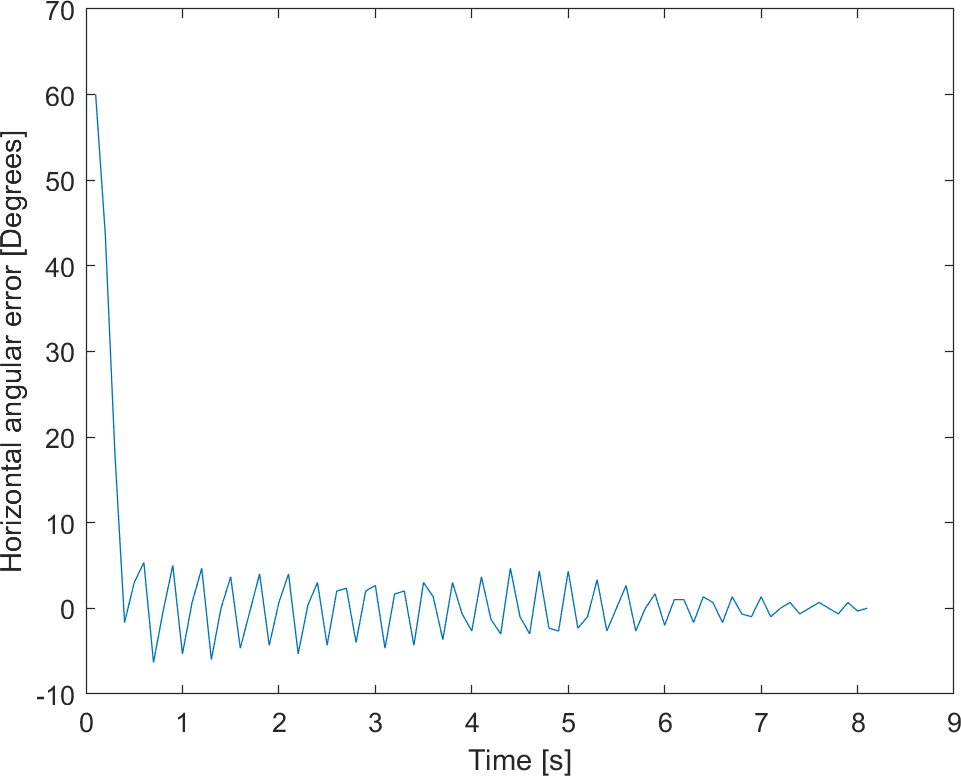
\includegraphics[width=\textwidth]{assets/Horizontal_undamped_oscillation.png}
\caption{Close to undamped oscillations from \(60^{\circ}\) step with P-controller.}
\label{Hor_osc}
\end{figure}
\subsection{Performance Of Line Follower}

\subsubsection{Test Setup}
Different types of controllers were made for the line following sequence.  A step response for the robot to follow was constructed as can be seen in fig. \ref{Step Response} The tests were made by letting the robot follow the straight black line which then turns with an angle of 37$^{\circ}$. The robot then follows the new direction of the line until it reach the perpendicular black line and stops. The angle was chosen to be 37$^{\circ}$, since it was determined that no steeper angles would be needed in the project. The initial idea was to use Ziegler Nichols method to tune a PID controller, but due to the fact that it was hard to reach a consistent oscillation on the line follower, this method was hard to implement. Instead P and PD controllers were tested and their performances were measured. PI and PID controllers were also tested, but the data from these tests was lost. It was determined that the controller that resulted in the smallest magnitude and amount of errors and had the shortest time with errors had the best performance. 


\begin{figure}[H]
    \centering
    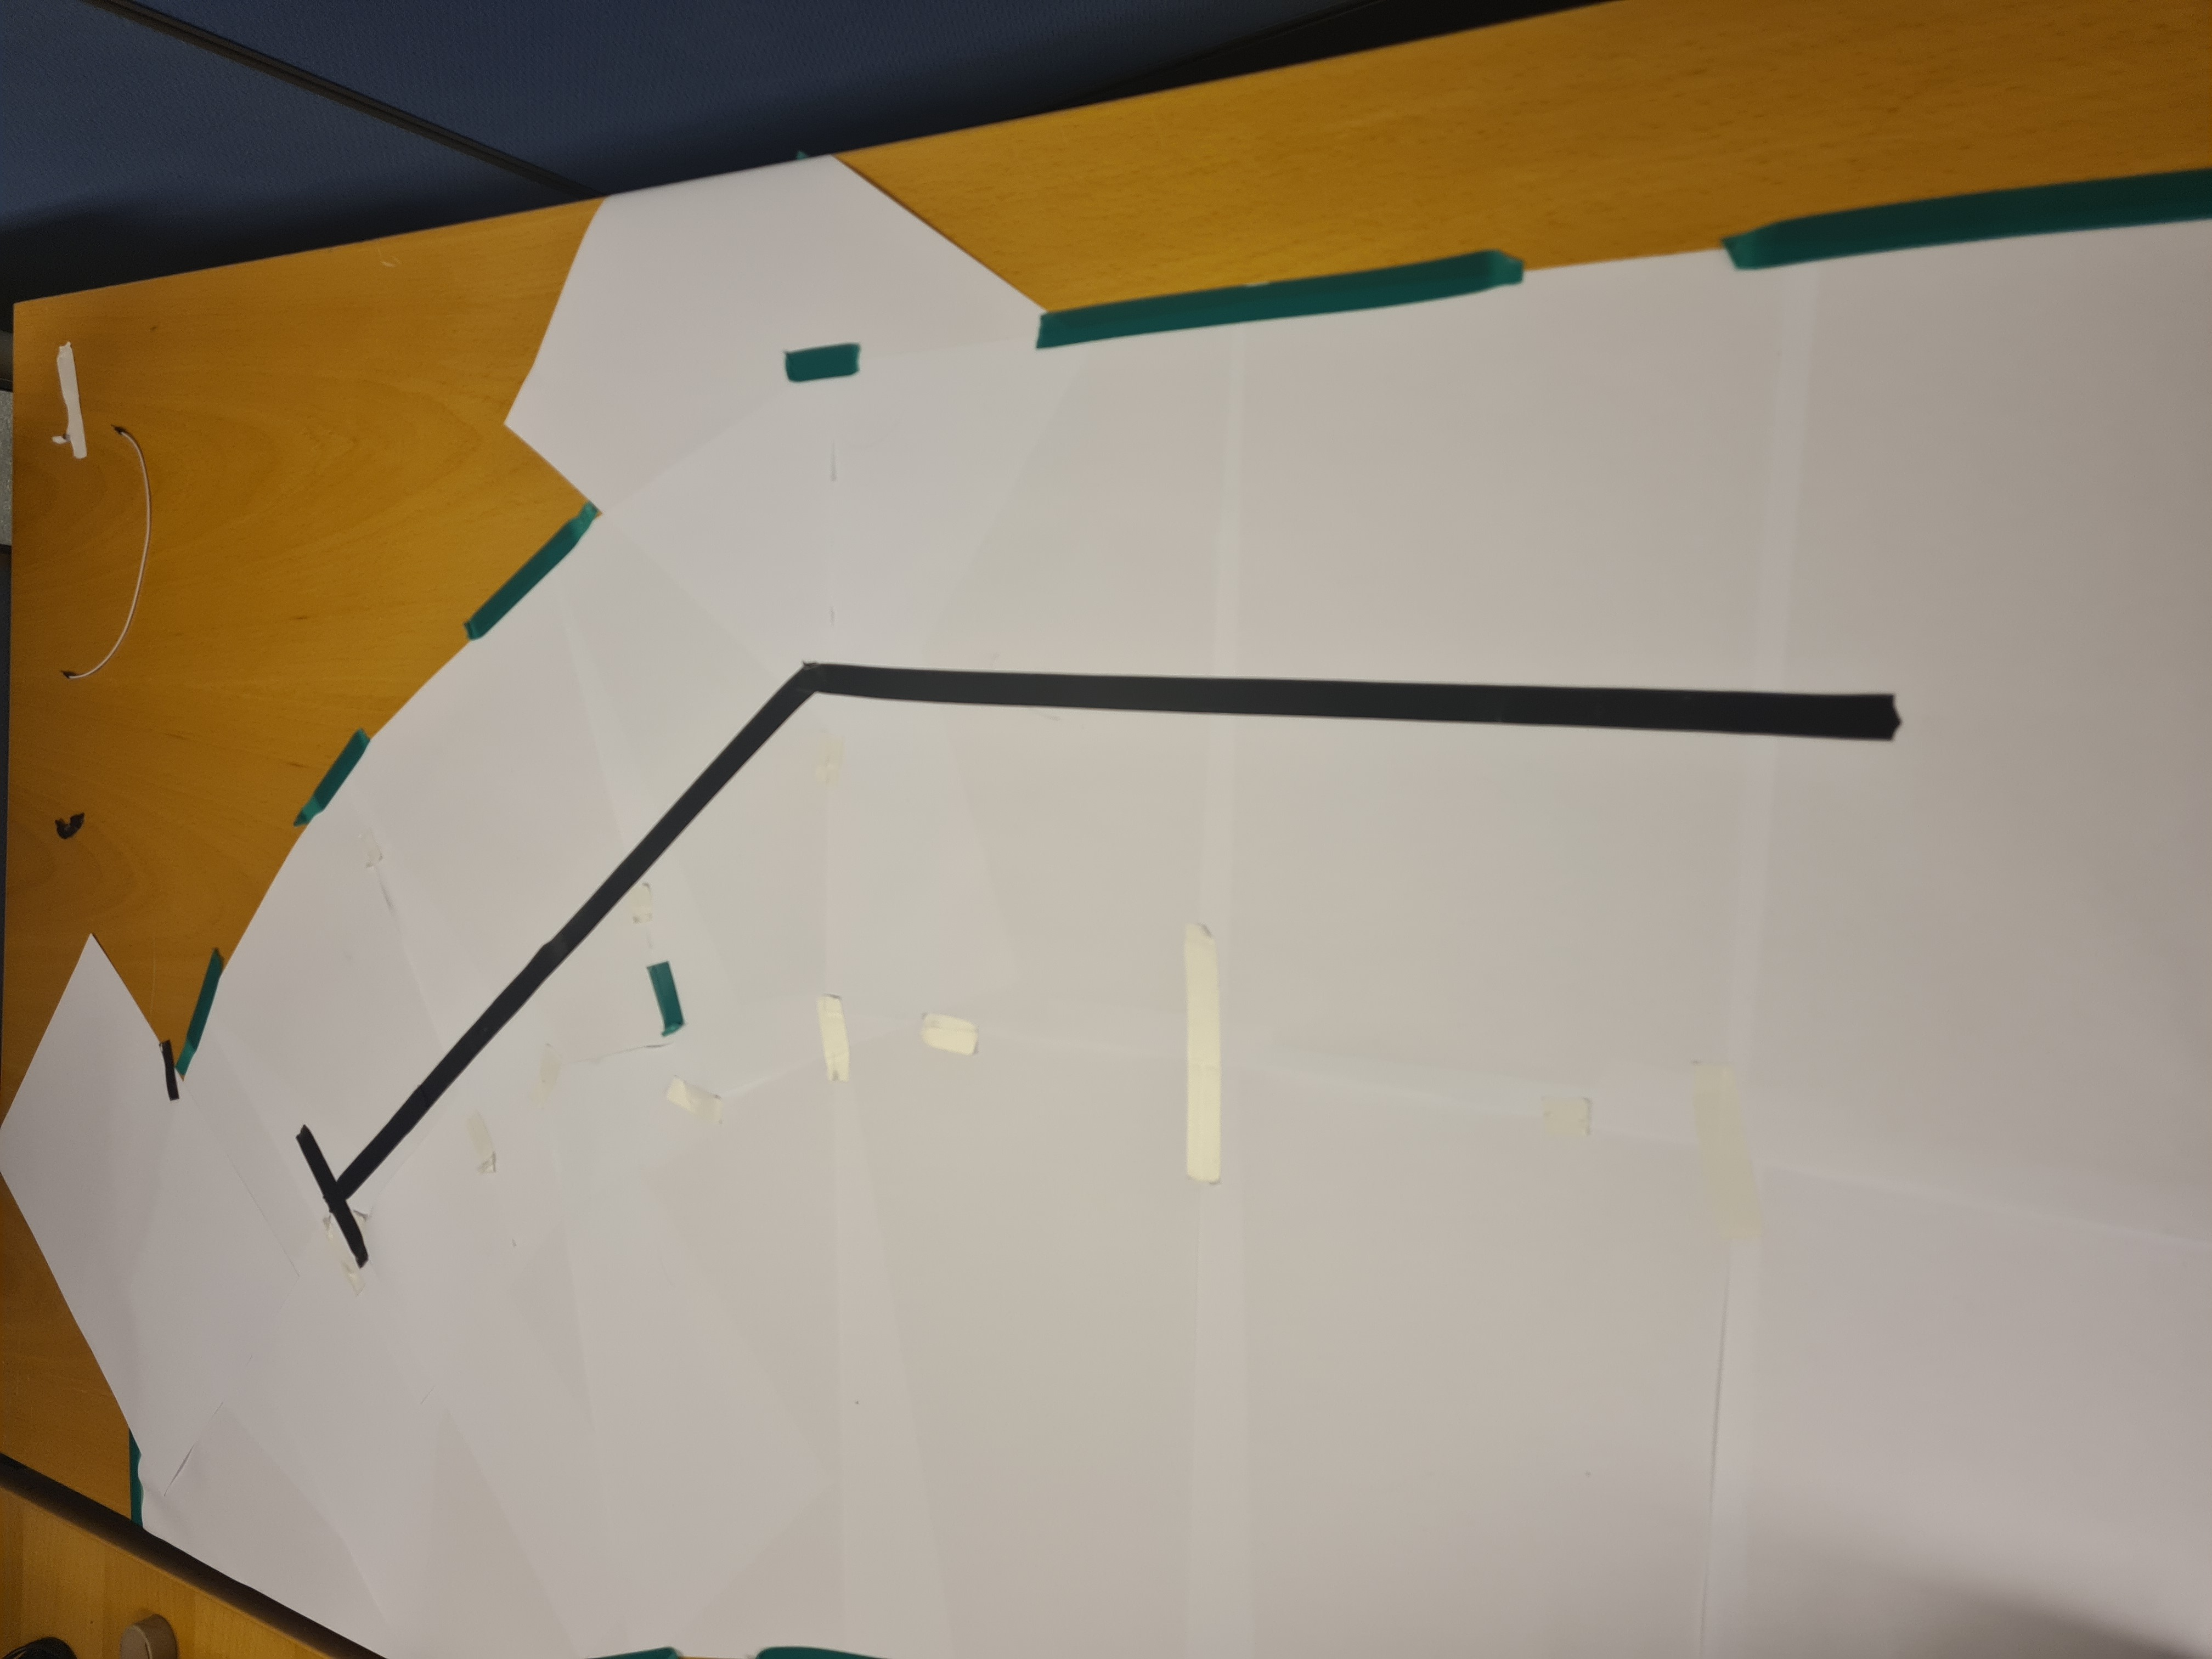
\includegraphics[width=\textwidth]{assets/Step Response.jpg}
    \caption{View of the line on which the step response was tested.}
    \label{Step Response}
\end{figure}

\subsubsection{P controller}
It was determined that the best P controller had the value of 40 on its Kp term. the performance of this controller during the step response can be sin in fig. \ref{Kp40}

\begin{figure}[H]
    \centering
    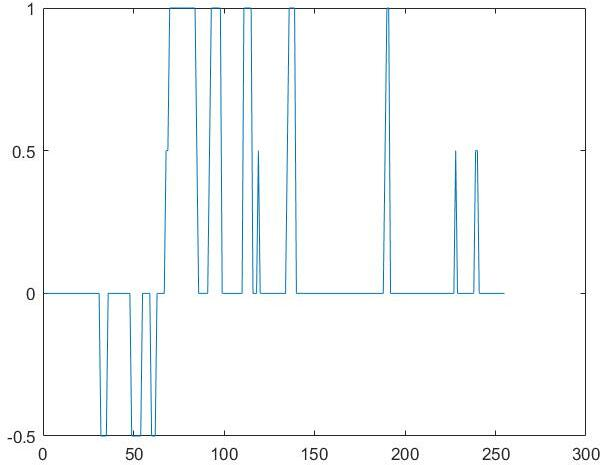
\includegraphics[width=\textwidth]{assets/Kp40.jpg}
    \caption{The error can be seen on the y-axis while the x axis represents the iteration of the loop.}
    \label{Kp40}
\end{figure}

\subsubsection{PD controller}
It was determined that the best PD controller had the value of 40 on its Kp term and 10 on the Kd-term. the performance of this controller during the step response can be sin in Fig. \ref{Kp40_10Kd}

\begin{figure}[H]
    \centering
    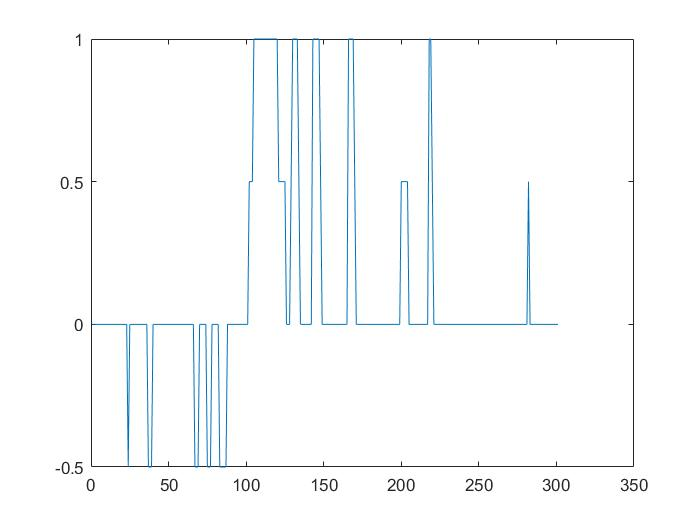
\includegraphics[width=\textwidth]{assets/Kp40_10Kd.jpg}
    \caption{The error can be seen on the y-axis while the x axis represents the iteration of the loop.}
    \label{Kp40_10Kd}
\end{figure}

\subsubsection{Conclusion}
Since the negative errors occurred before the turn, and were likely caused by a poor placement of the robot in the start of the experiment, these errors were not taken into account when determining the quality of the controllers. It was thus determined that the PD-controller performed a bit better than the P-controller, it had fewer error spikes and they lasted for a shorter period of time. More importantly, the spikes were lesser frequent at the end of the experiment.
